Based on simulations with the Inundation Model and analysis of the results, the results of the 2023 storm surge simulation and future storm surges for a statistical 100-year event and a projected storm surge in SSP4.5 and 8.5 emission scenario are presented. The results of the simulated storm surge are compared with the observed extent of the storm surge.

\subsection{Simulated 2023-storm surges}
Figure \ref{Subfig: Målt Aabenraa} shows the inundated map prepared by Aabenraa municipality, showing the extent of the observed storm surge and figure \ref{Subfig: Model Aabenraa} shows the result of the simulation for Aabenraa.
\begin{figure}[H]
\begin{subfigure}[t]{0.5\textwidth}
	\centering
	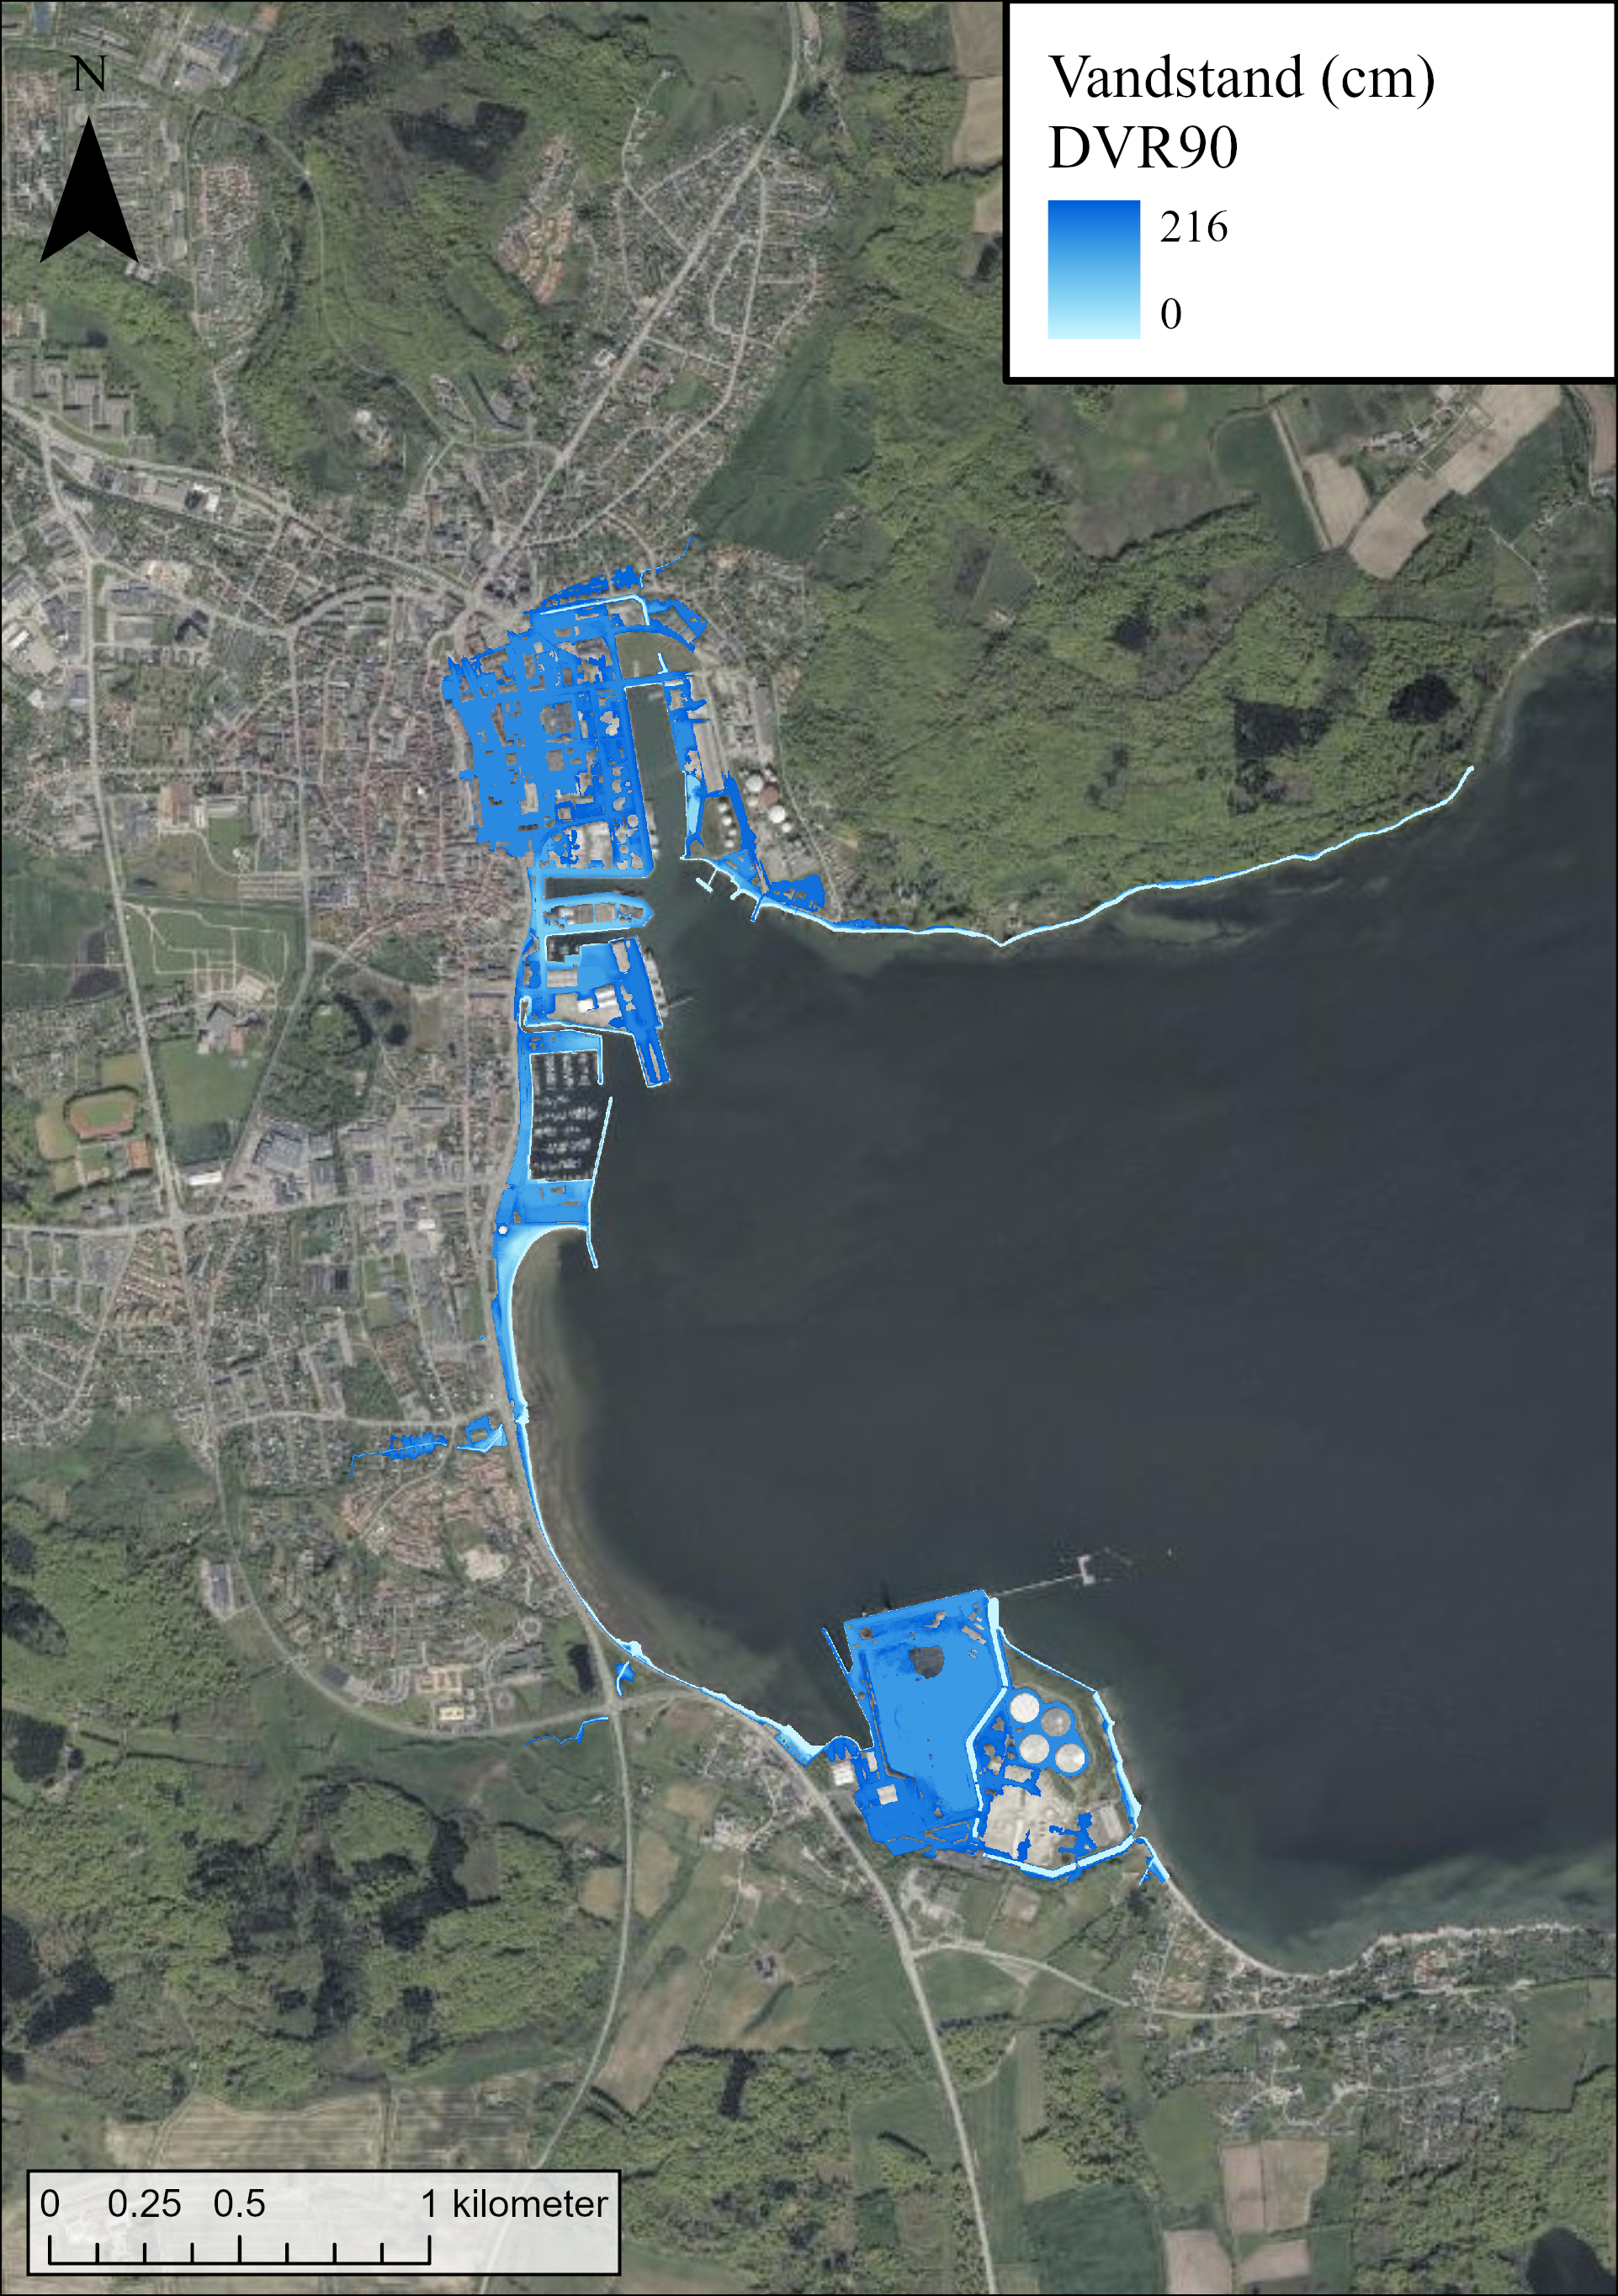
\includegraphics[width=0.95\linewidth]{images/Resultater/2023Malt/2023 resultat_aabenraa.jpg}
	\caption{}
	\label{Subfig: Målt Aabenraa}
\end{subfigure}
\begin{subfigure}[t]{0.5\textwidth}
	\centering
	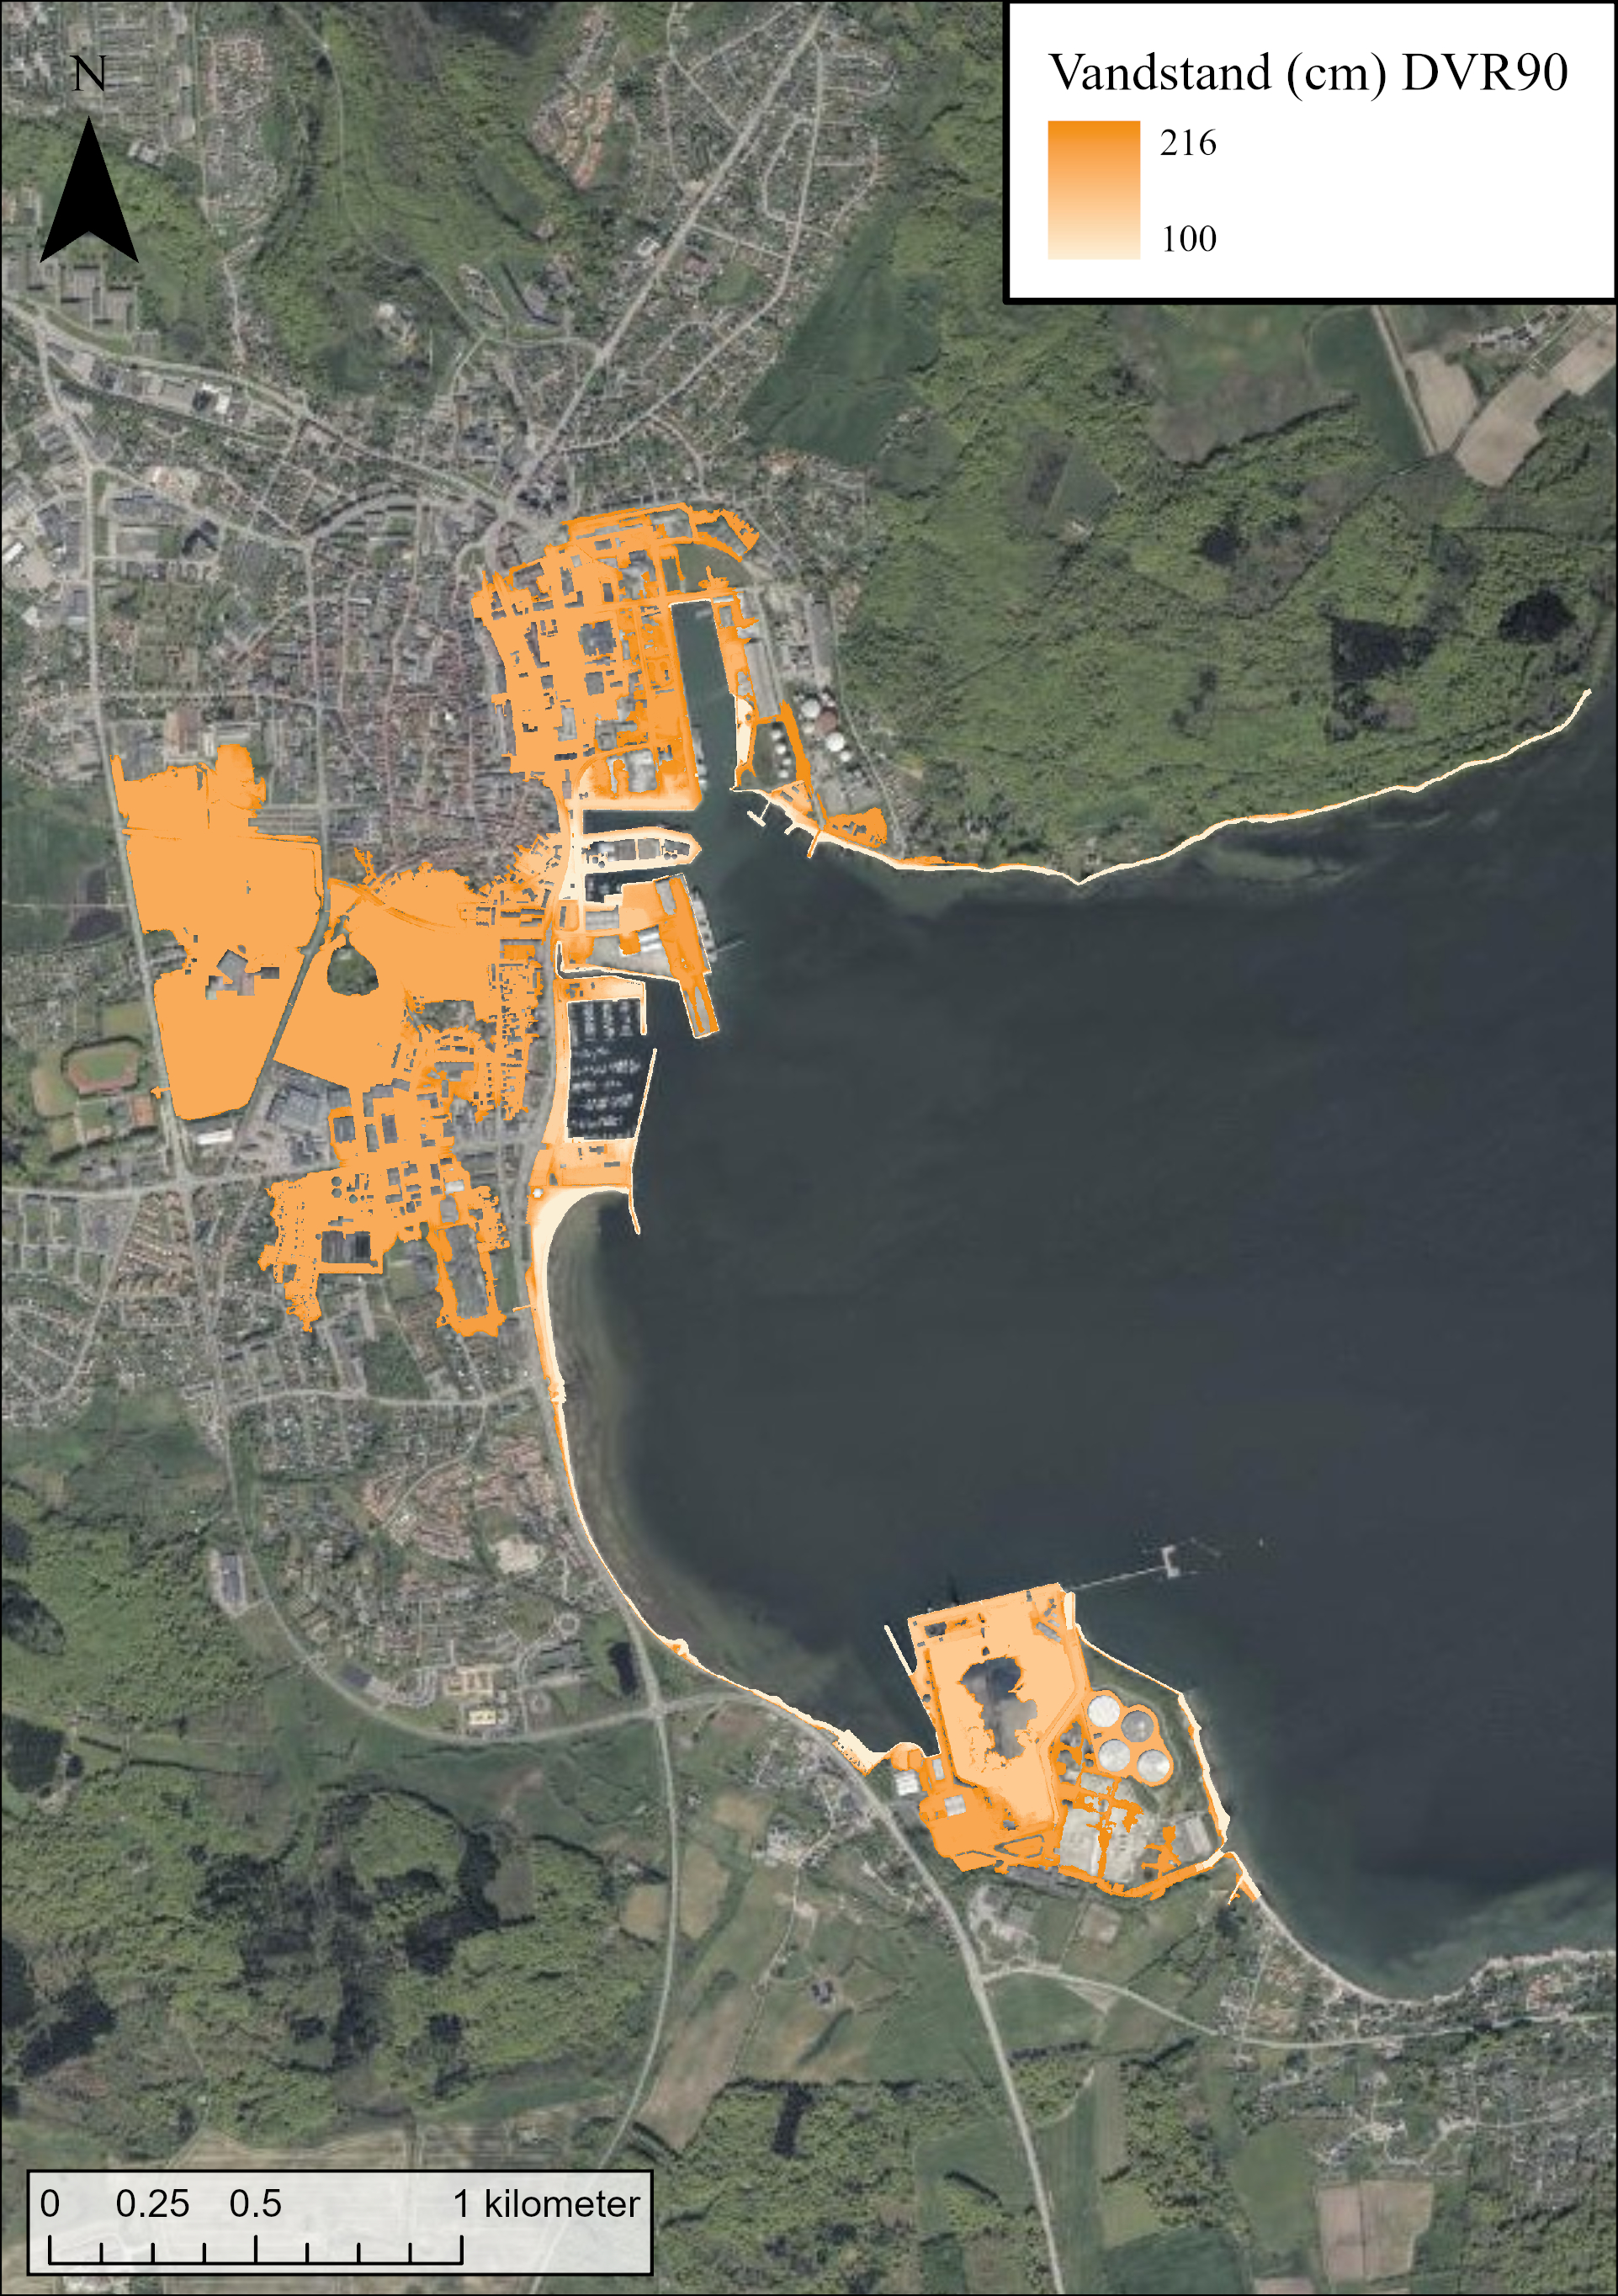
\includegraphics[width=0.95\linewidth]{images/Resultater/2023Model/2023 model_aabenraa.jpg}
	\caption{}
	\label{Subfig: Model Aabenraa}
\end{subfigure}
\caption{Oversvømmelseskort over 2023-stormfloden for Aabenraa. \textbf{(a)} Observeret data \textbf{(b)} Simuleret data.}
\label{Figur: Målt & simuleret Aabenraa}
\end{figure}
There is a difference between the two maps. The model result is larger, especially west of the marina at a mixed recreational and built-up area. The model resulted in an inundated area of 129.8 hectares, while the observed area was 70.1 hectares. This means that the model's result is 83.5\% larger than the observed extent, corresponding to approximately 59 hectares.\\

\begin{figure}[H]
	\begin{subfigure}[t]{0.5\textwidth}
		\centering
		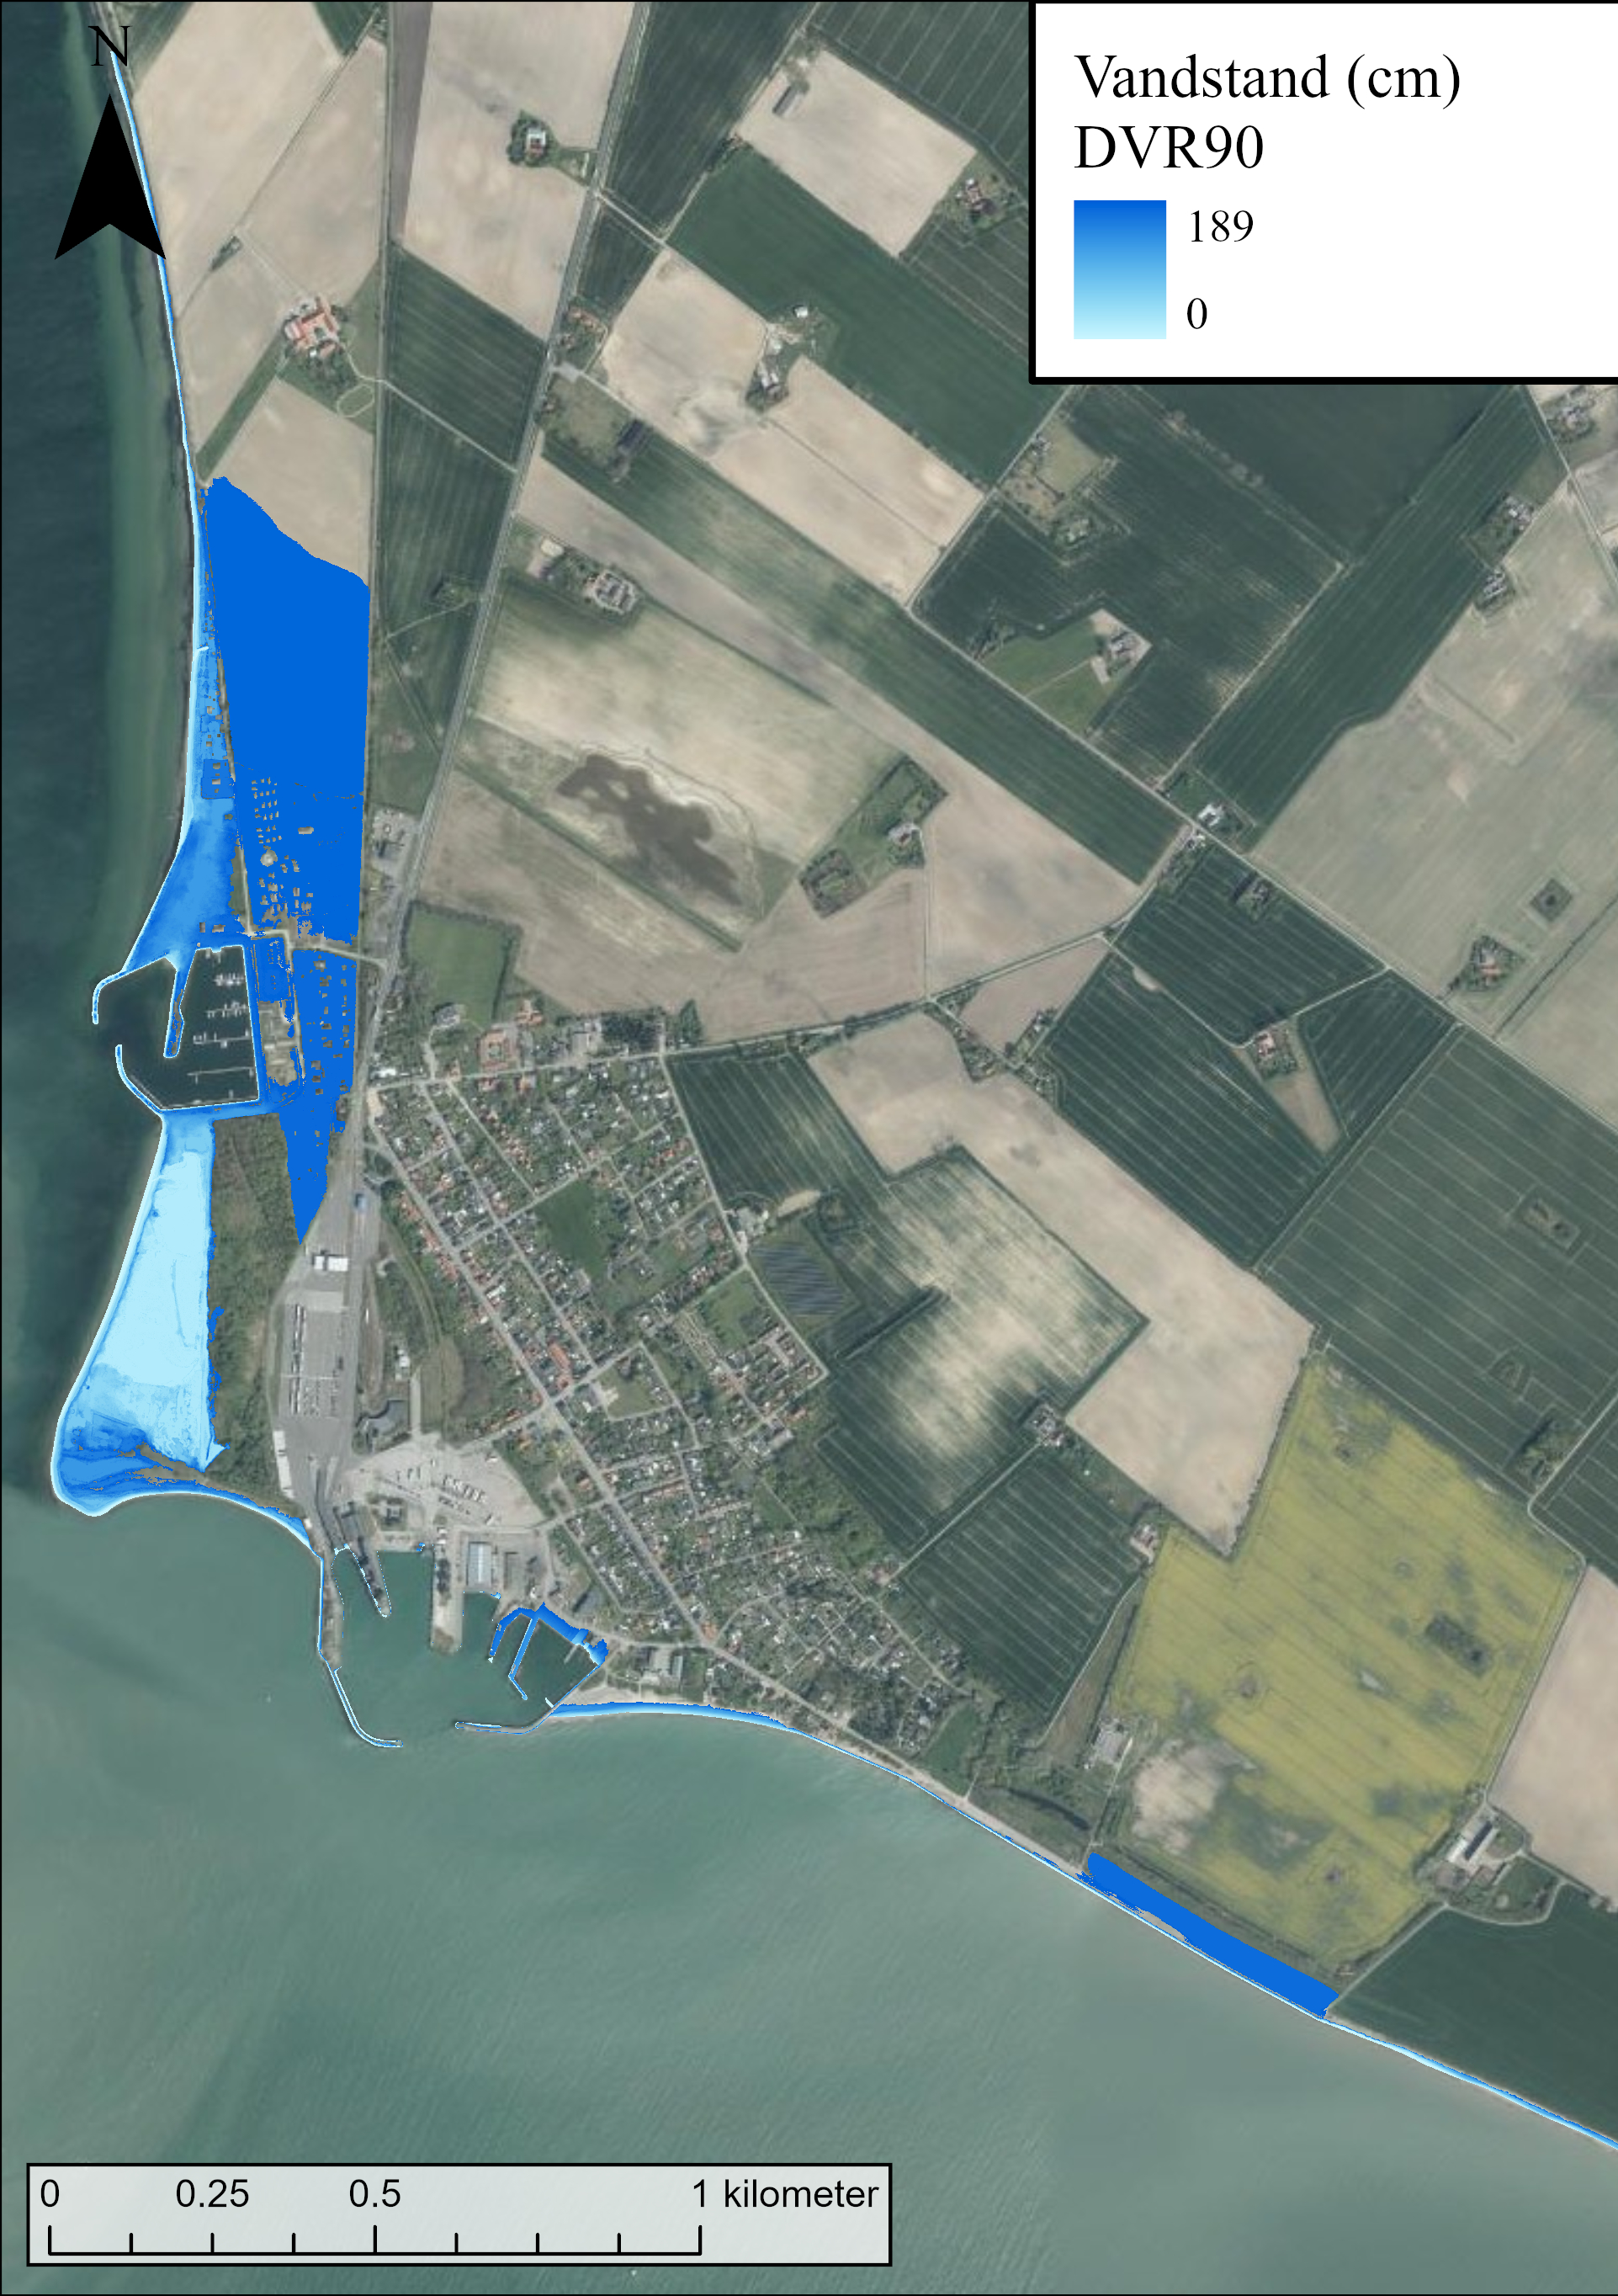
\includegraphics[width=0.95\linewidth]{images/Resultater/2023Malt/2023 resultat_gedser.jpg}
		\caption{}
		\label{Subfig: Målt Gedser}
	\end{subfigure}
	\begin{subfigure}[t]{0.5\textwidth}
		\centering
		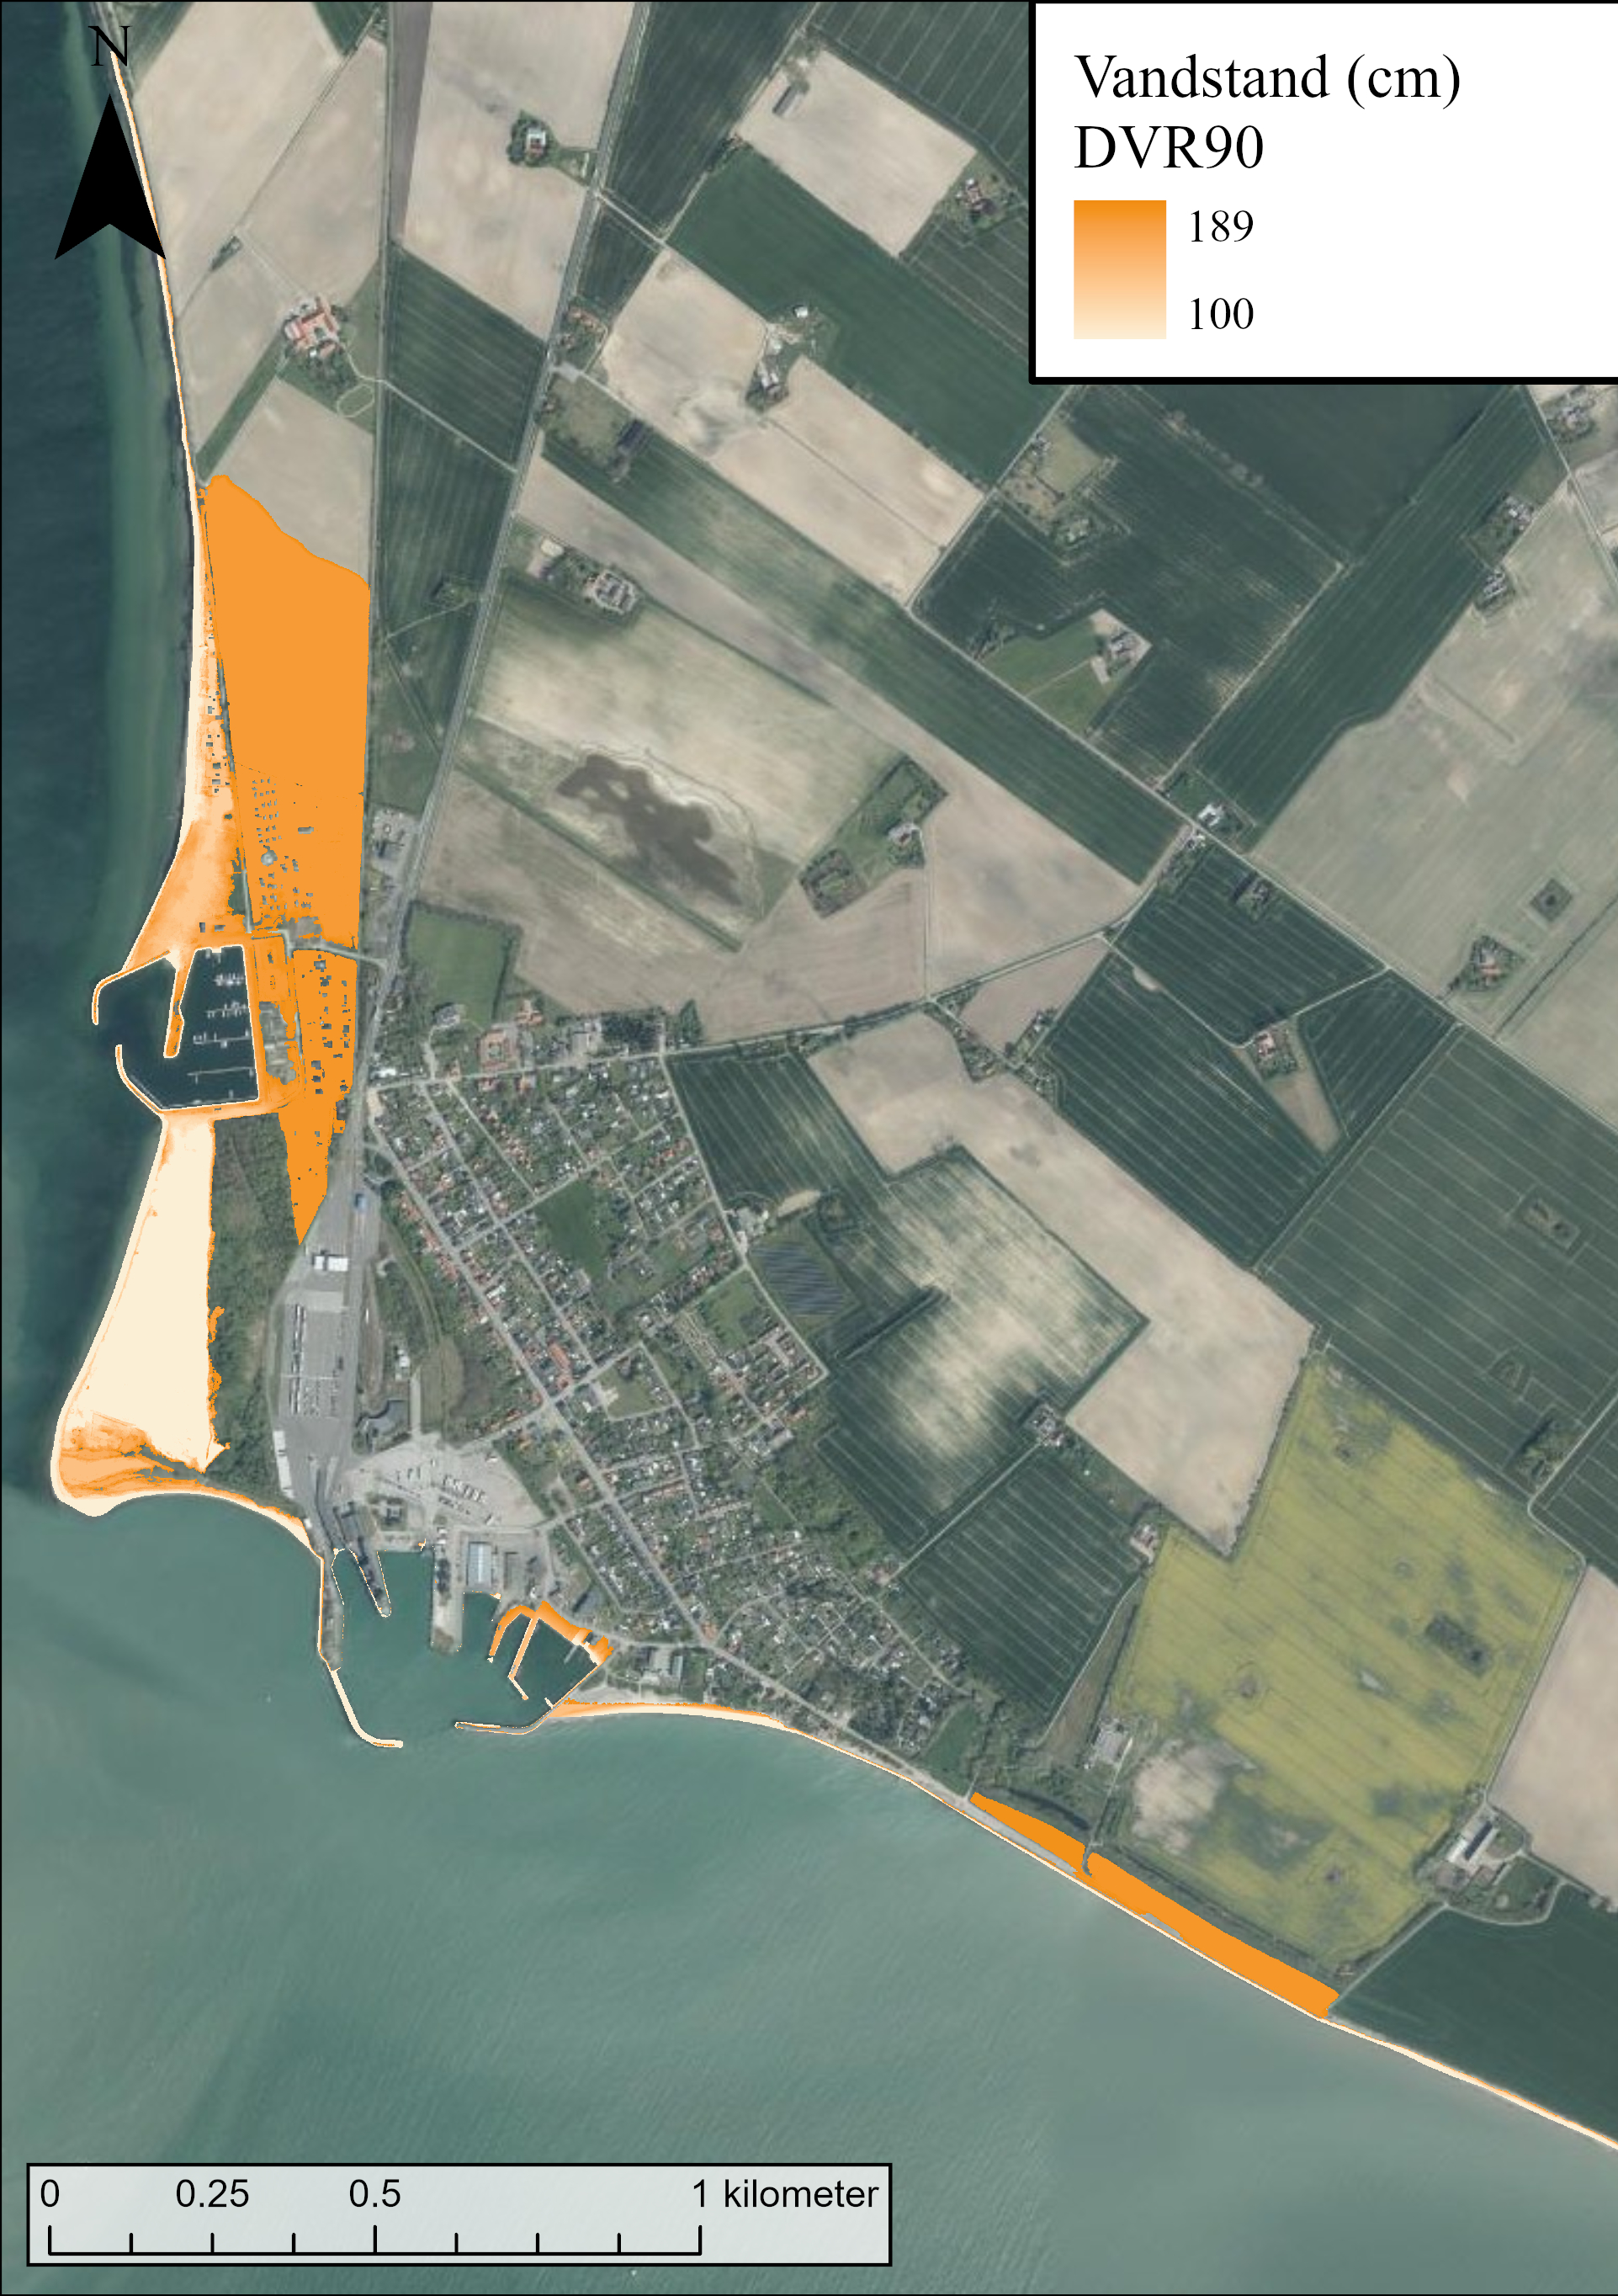
\includegraphics[width=0.95\linewidth]{images/Resultater/2023Model/2023 model_gedser.jpg}
		\caption{}
		\label{Subfig: Model Gedser}
	\end{subfigure}
	\caption{Oversvømmelseskort over 2023-stormfloden for Gedser Havn. \textbf{(a)} Observeret data. \textbf{(b)} Simuleret data}
	\label{Figur: Målt & simuleret Gedser}
\end{figure}
Figure \ref{Subfig: Målt Gedser} shows the inundated area of the observed storm surge for Gedser Havn. Figure \ref{Subfig: Model Gedser} shows the simulated result. The result from the Inundation Model is the same as the observed extent. The observed event had a flooded area of 34.5 hectares compared to 33.2 hectares from the Inundation Model. The model's result is therefore approximately 4\% smaller, corresponding to approximately 1.3 hectares. It is primarily the area around the marina north of the ferry port and a low-lying nature area west of the ferry port that was flooded. This is evident from both observed data and the simulated result.\\

\begin{figure}[H]
	\begin{subfigure}[t]{0.5\textwidth}
		\centering
		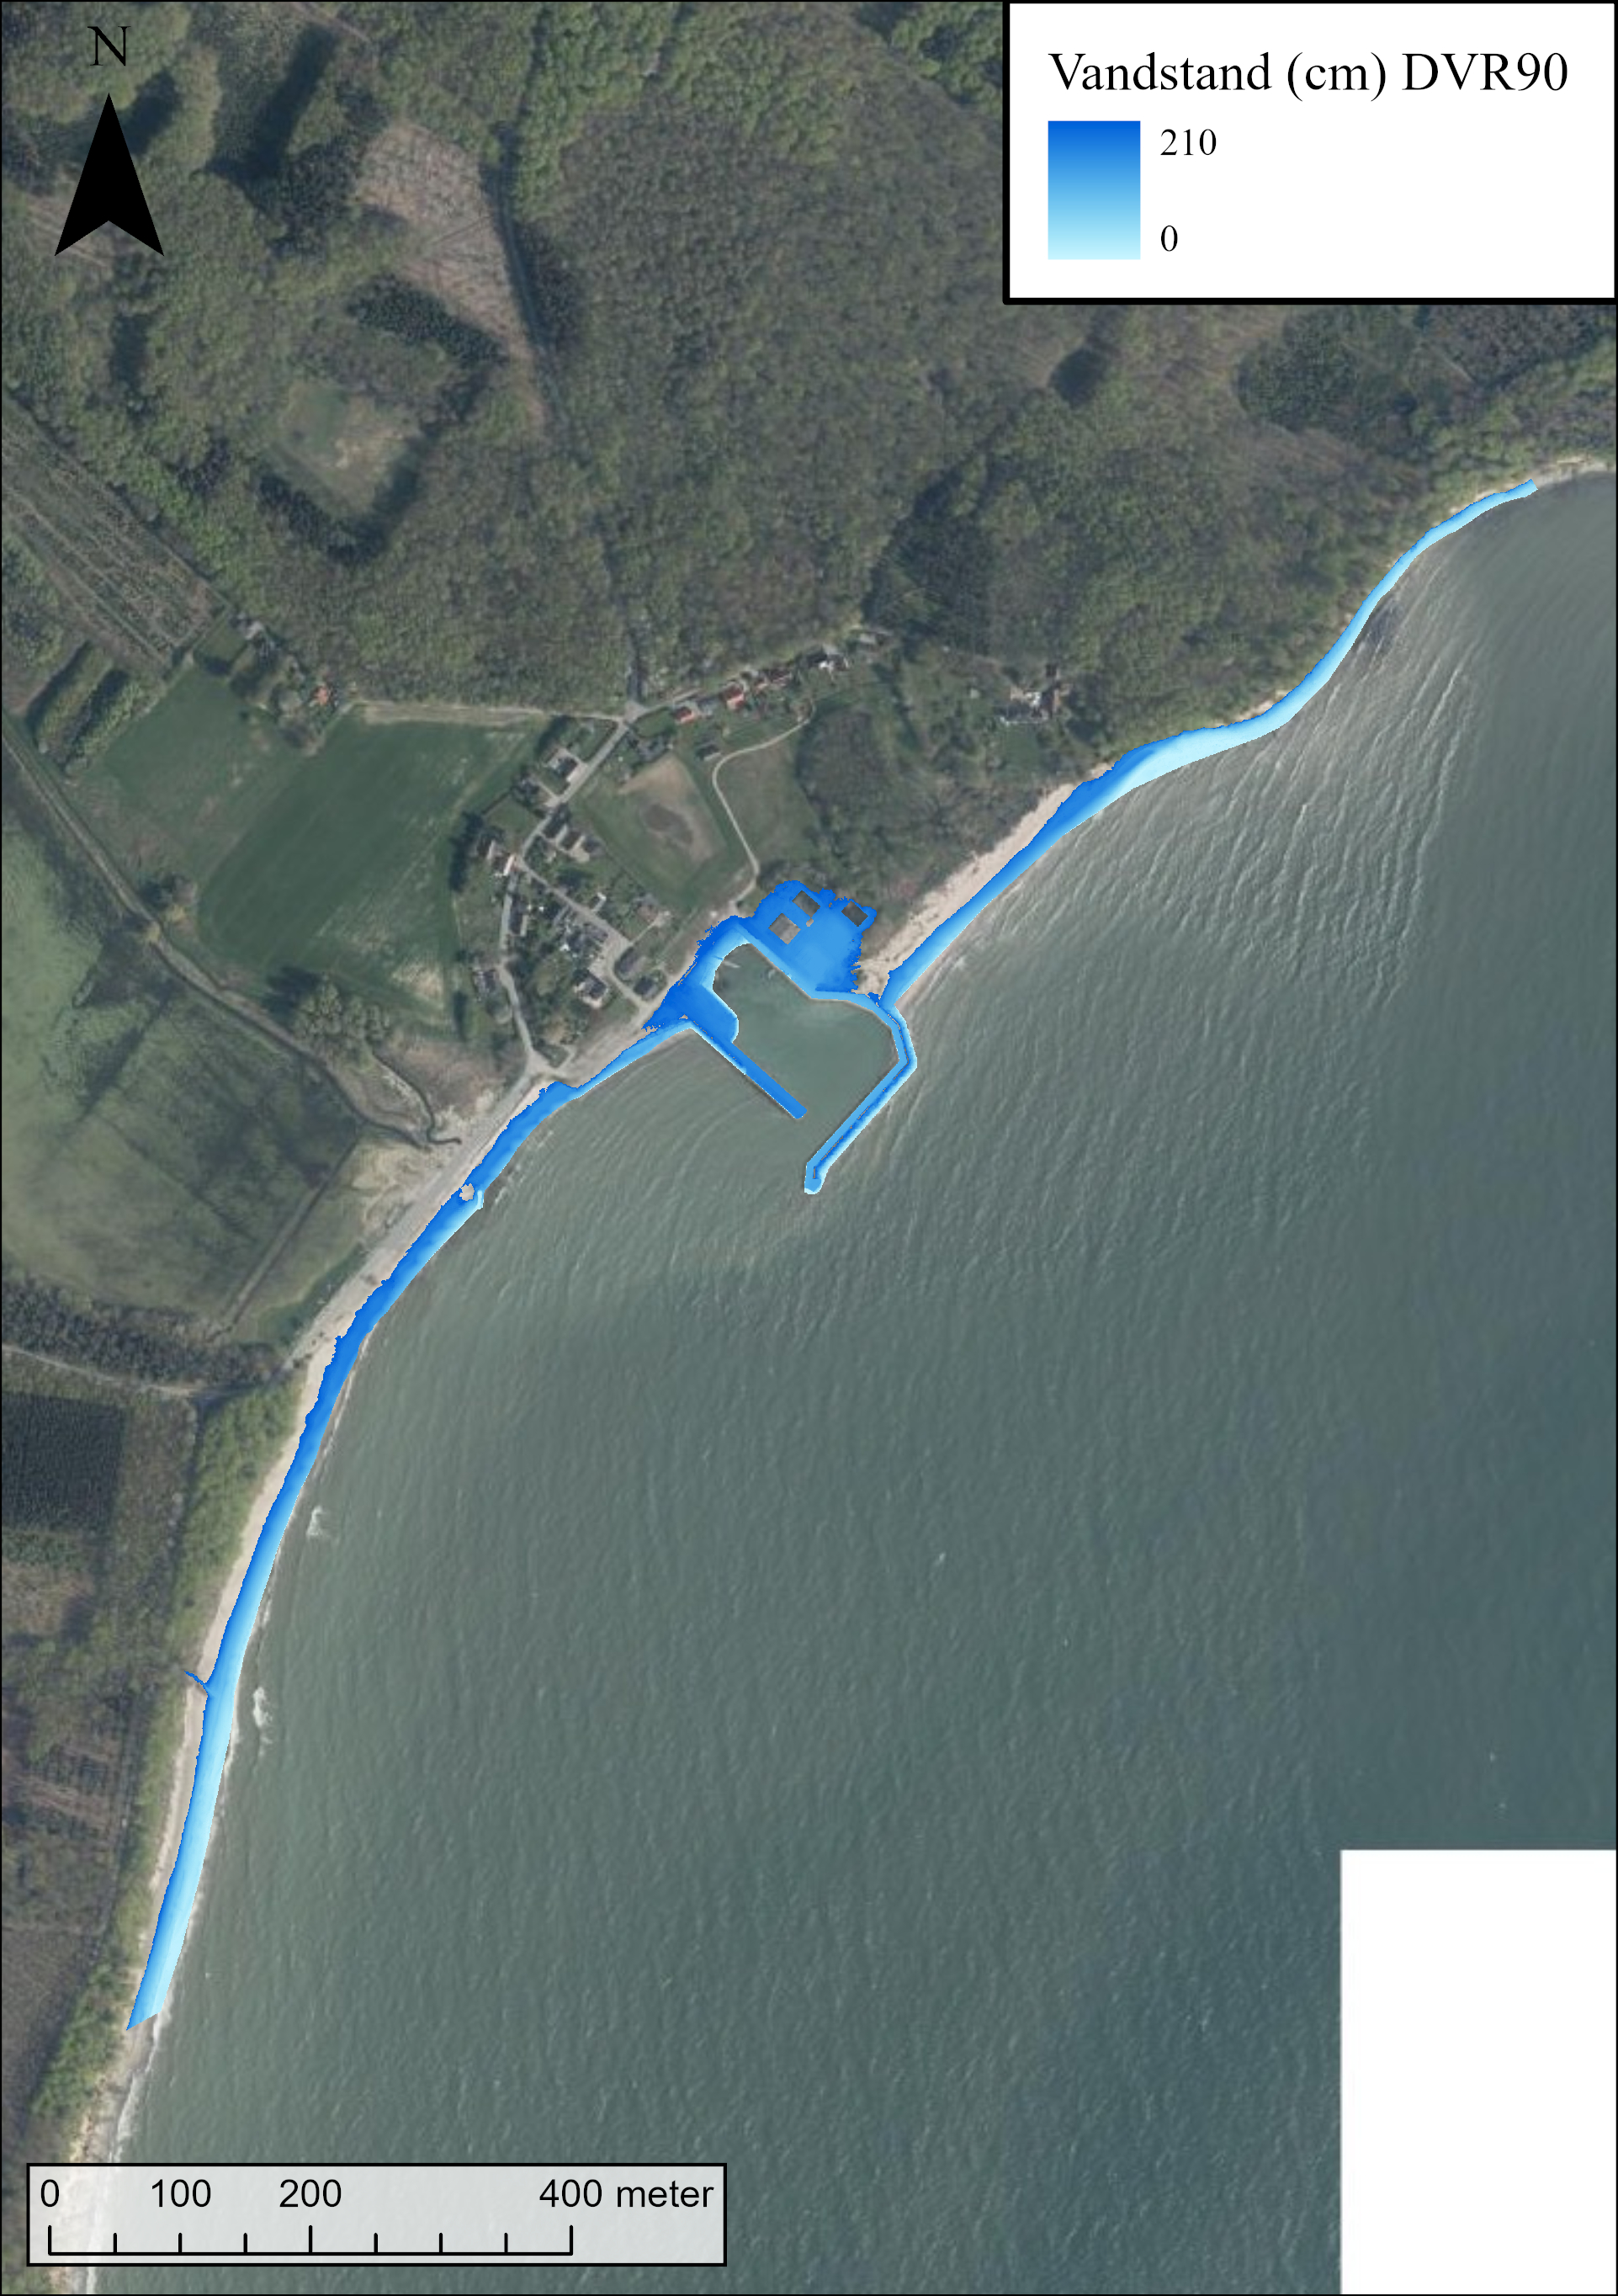
\includegraphics[width=0.95\linewidth]{images/Resultater/2023Malt/2023 resultat_hesnaes.jpg}
		\caption{}
		\label{Subfig: Målt Hesnæs}
	\end{subfigure}
	\begin{subfigure}[t]{0.5\textwidth}
		\centering
		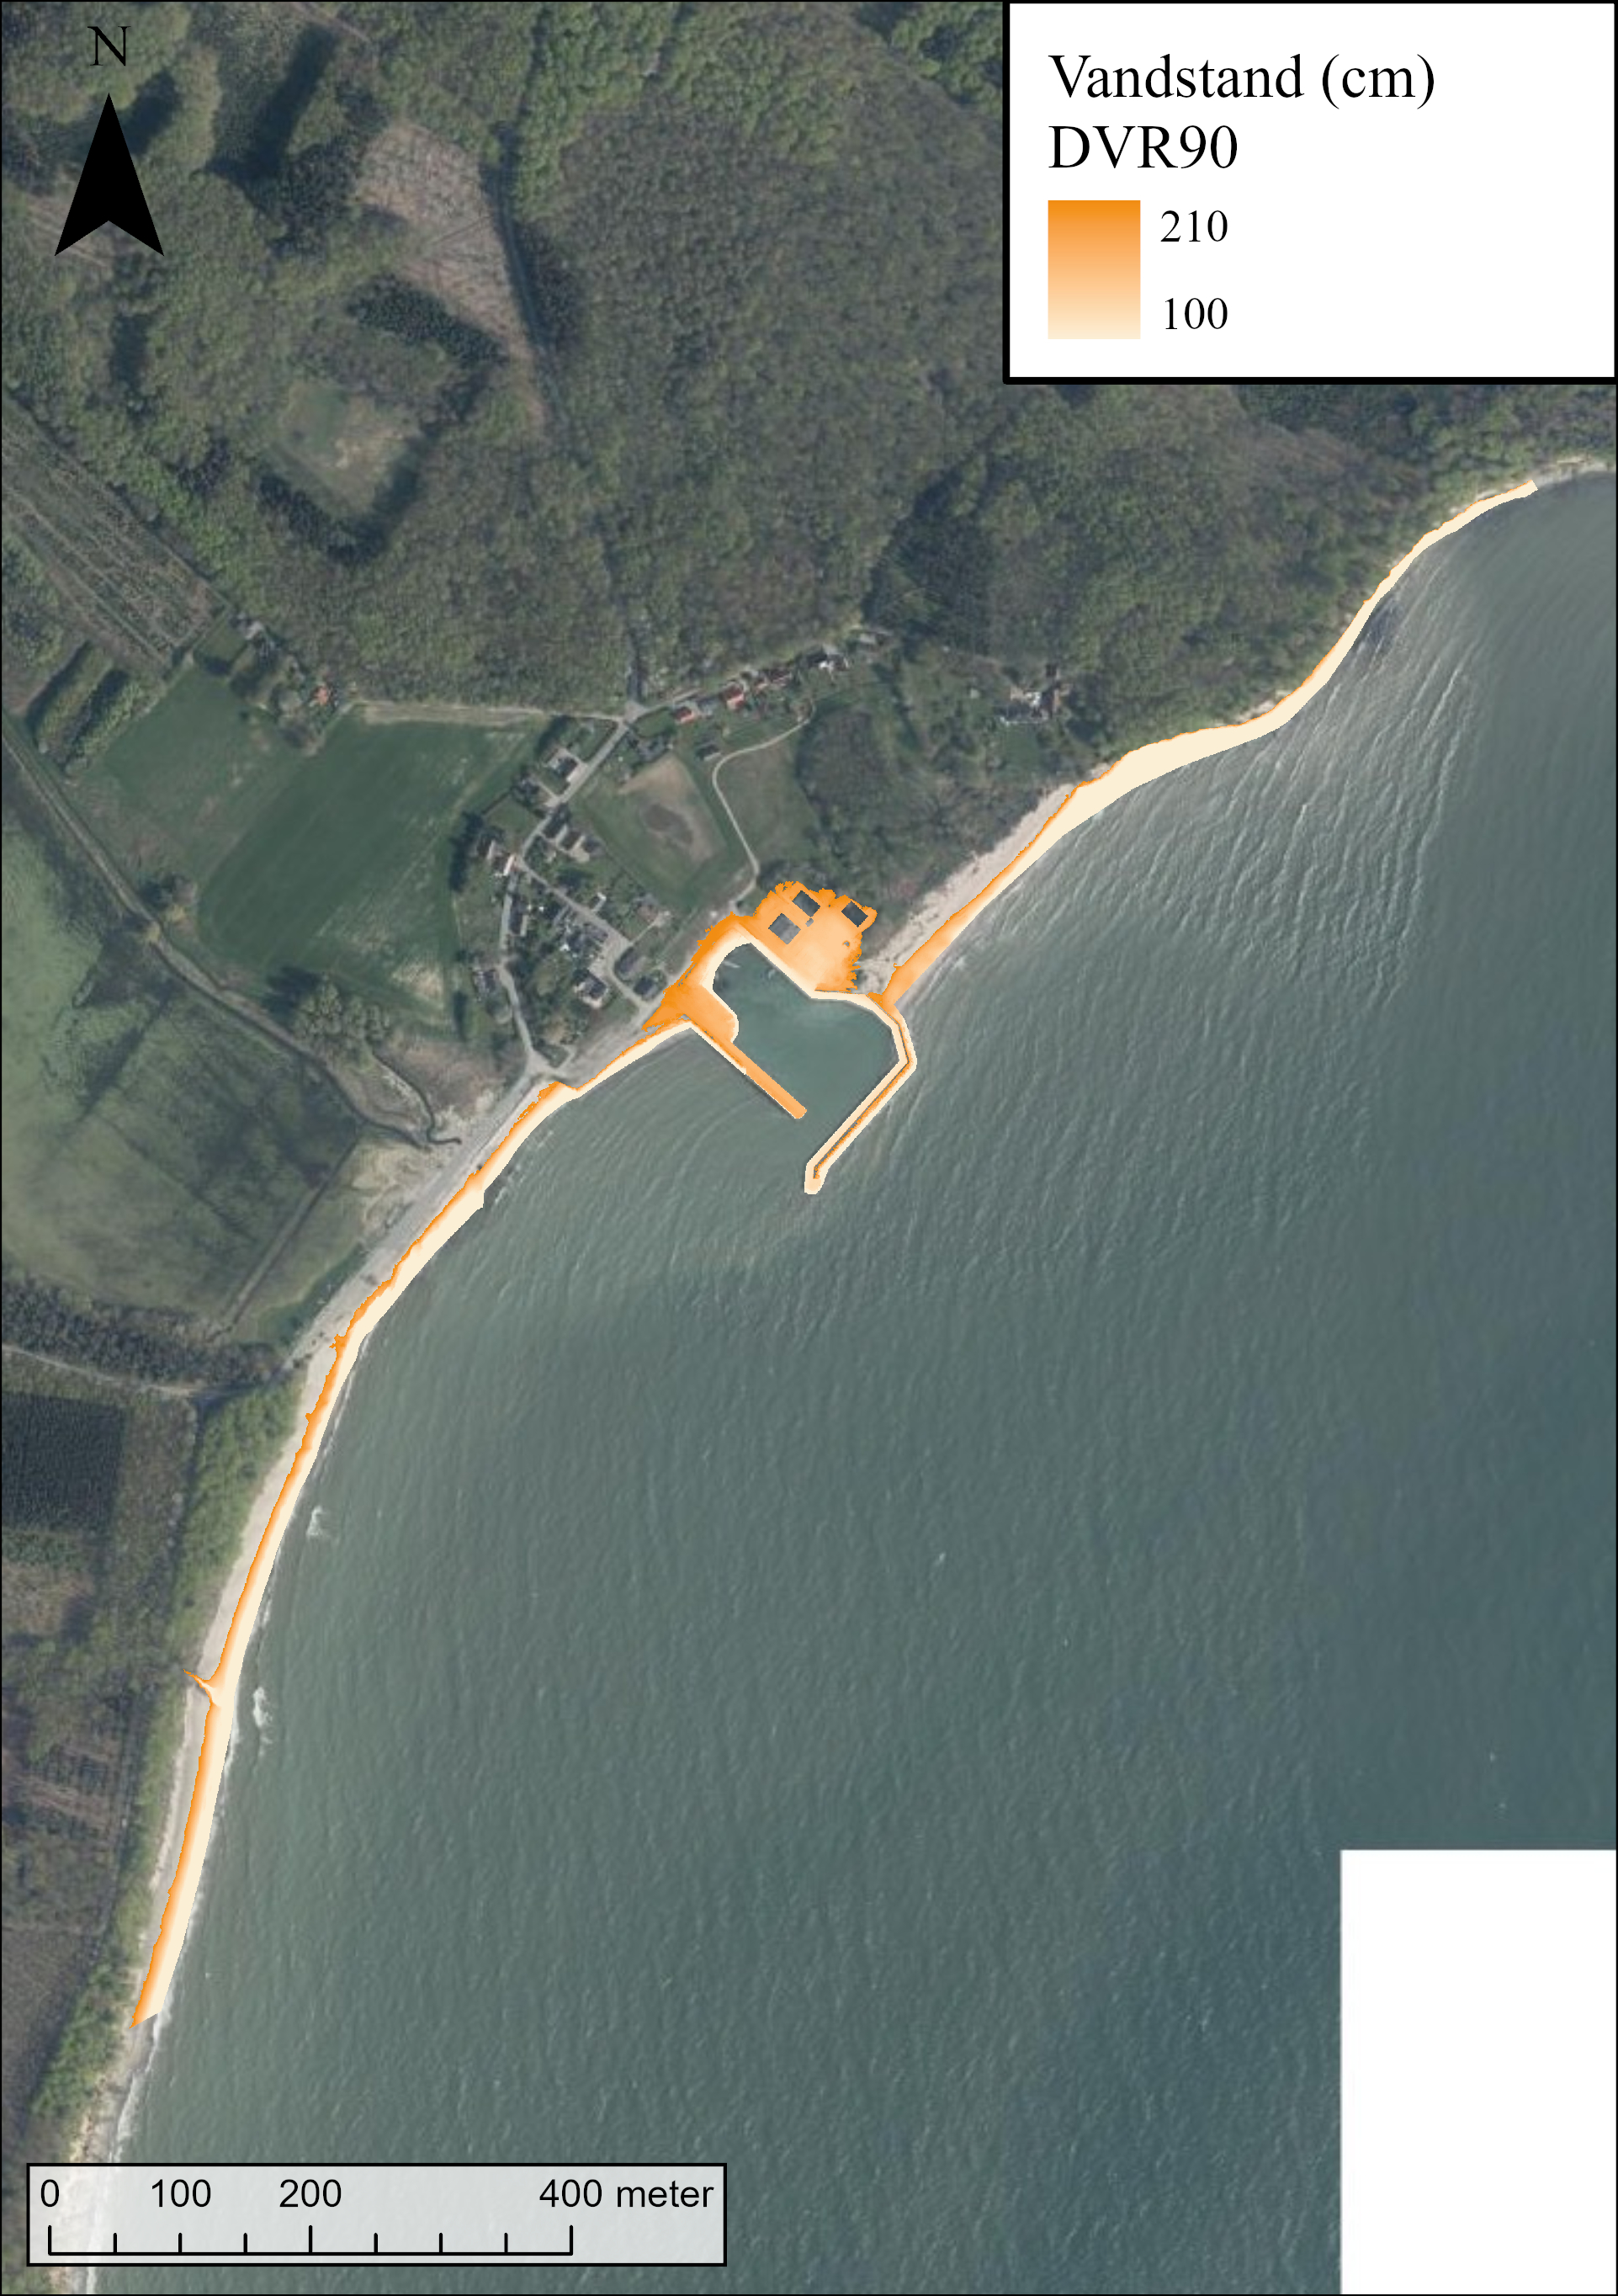
\includegraphics[width=0.95\linewidth]{images/Resultater/2023Model/2023 model_hesnaes.jpg}
		\caption{}
		\label{Subfig: Model Hesnæs}
	\end{subfigure}
	\caption{Oversvømmelseskort over 2023-stormfloden for Hesnæs. \textbf{(a)} Observeret data. \textbf{(b)} Simuleret data.}
	\label{Figur: Målt & simuleret Hesnæs}
\end{figure} 
For Hesnæs, it was primarily the harbour, including the harbour pier and the coastline that was flooded during the storm surge (figure \ref{Subfig: Målt Hesnæs}). The result from the Inundation Model in figure \ref{Subfig: Model Hesnæs} gives the same result and there is minimal difference between the two maps. The observed extent had an inundated area of 3.5 hectares and the simulated result had an extent of 3.3 hectares. The model's result is therefore 0.2 hectares smaller, corresponding to a difference of 5.2\%.\\

\begin{figure}[H]
	\begin{subfigure}[t]{0.5\textwidth}
		\centering
		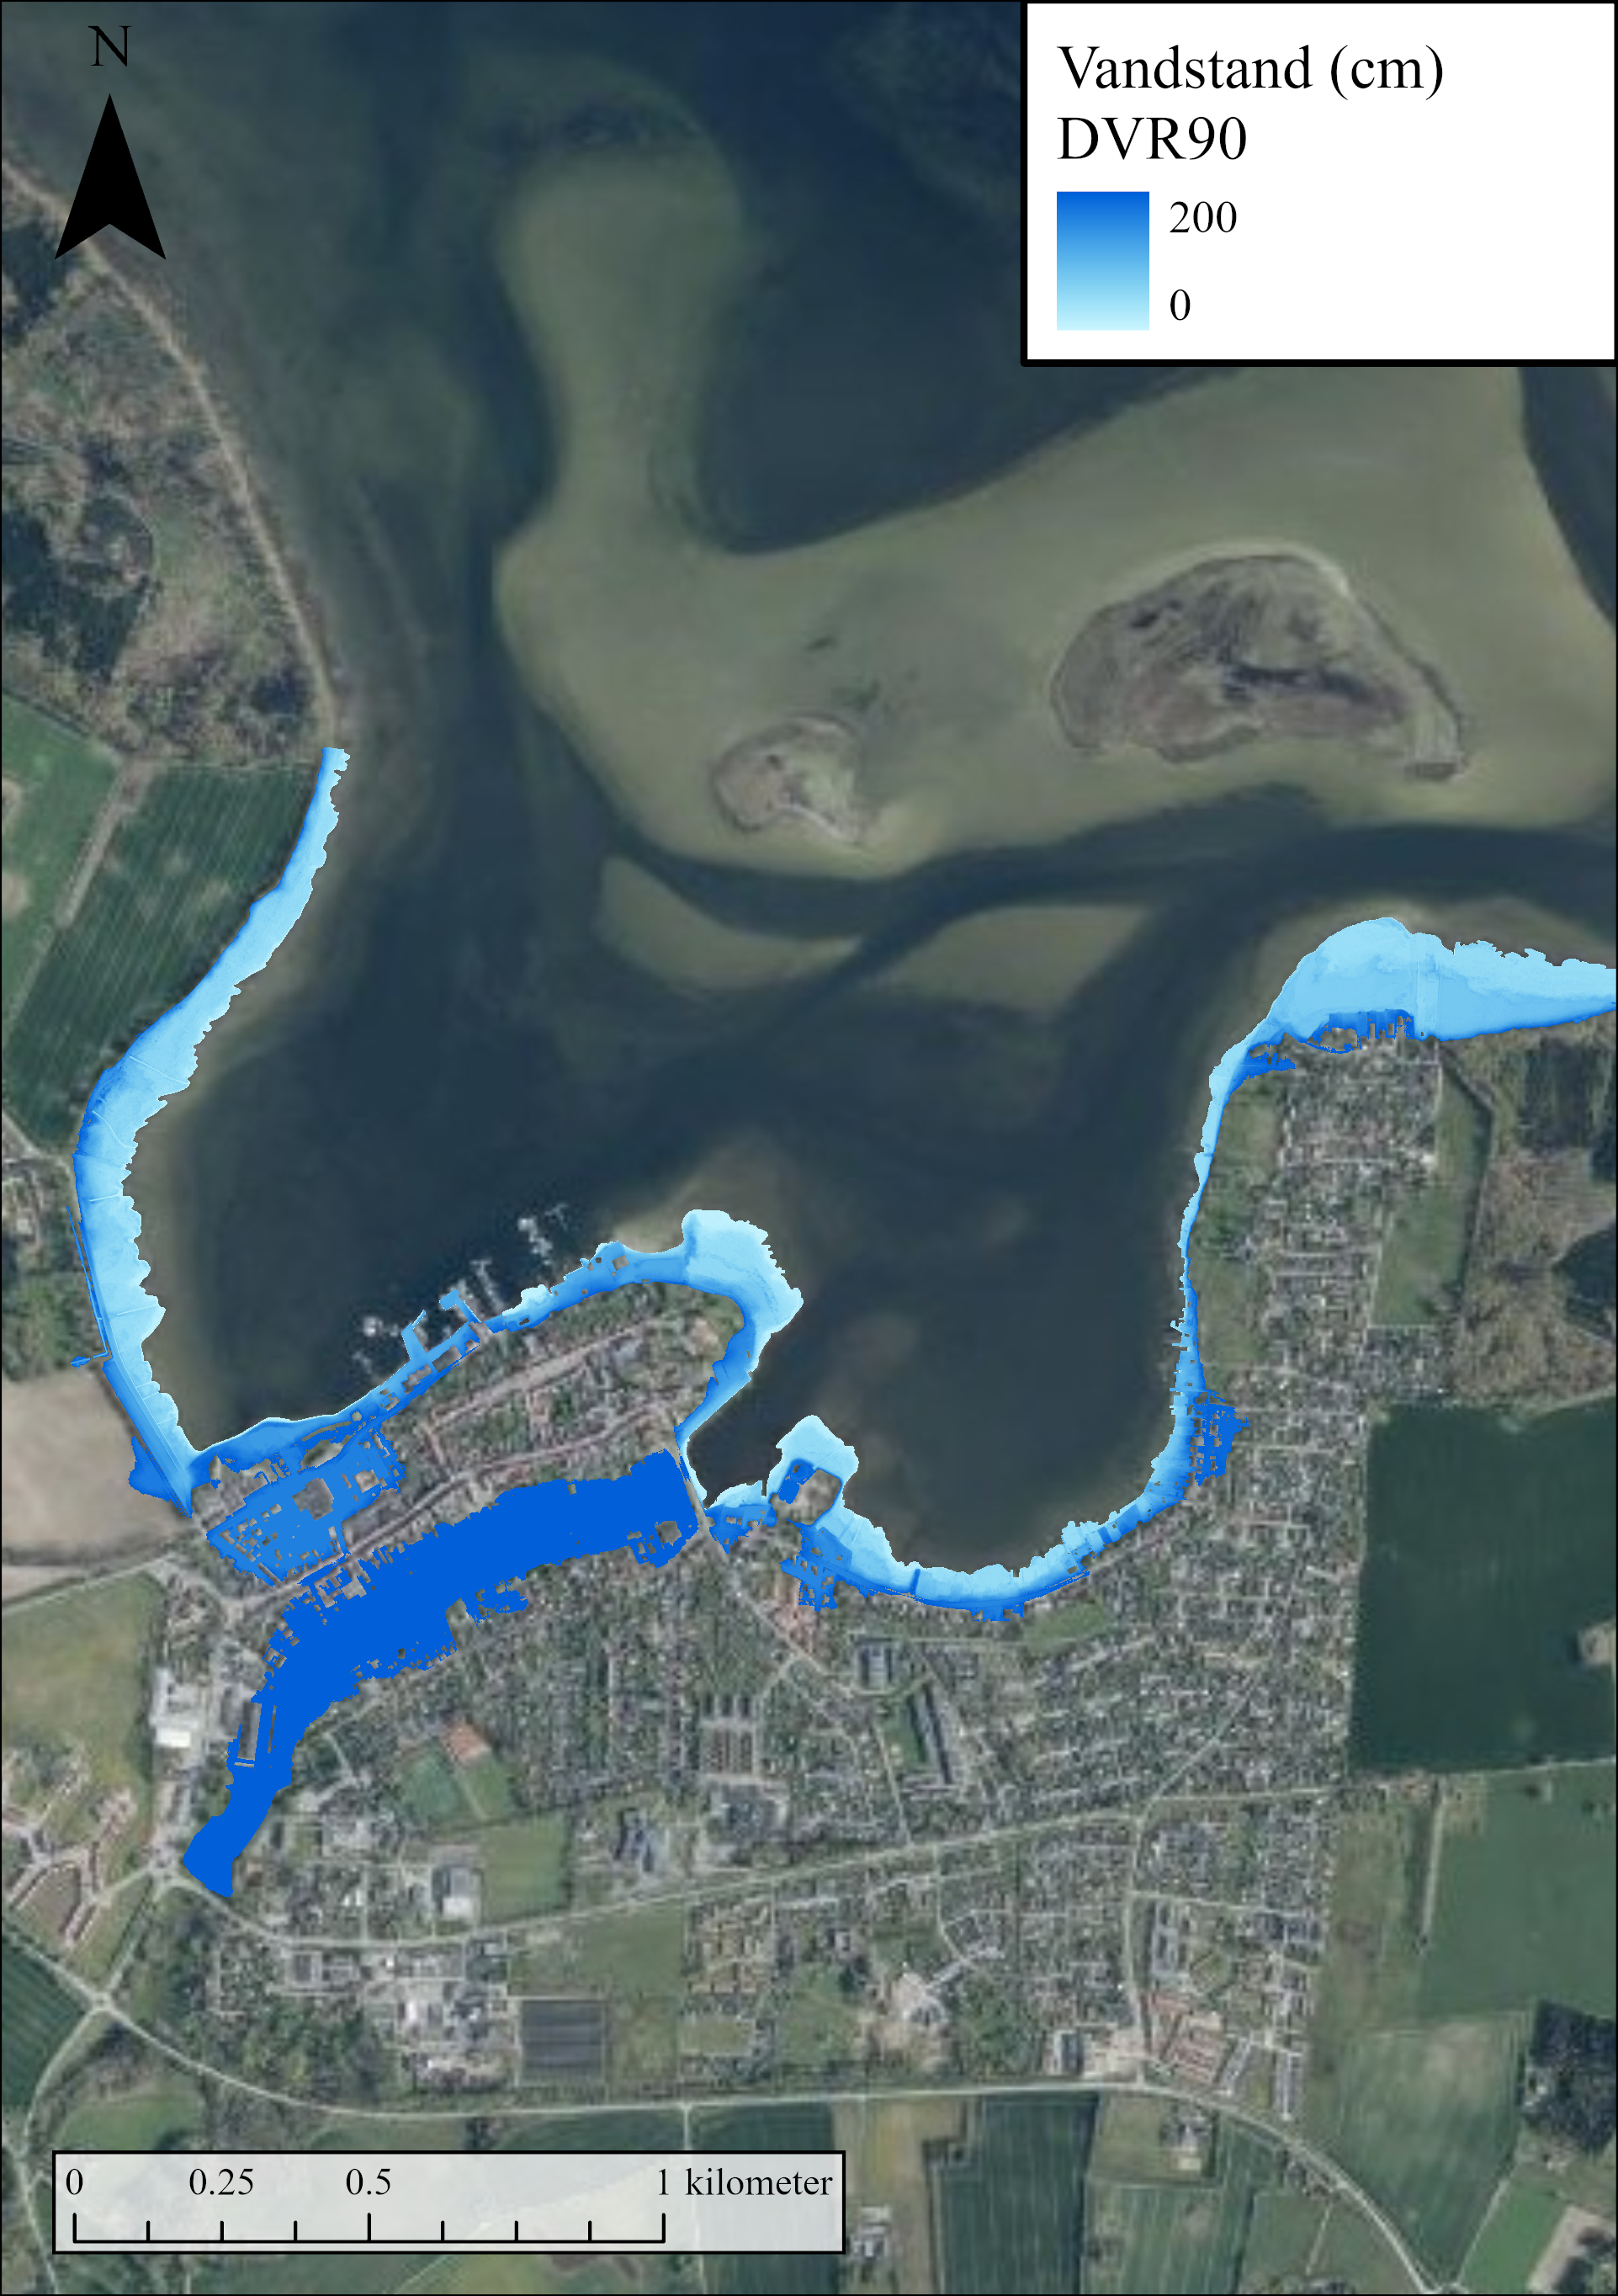
\includegraphics[width=0.95\linewidth]{images/Resultater/2023Malt/2023 resultat_praestoe.jpg}
		\caption{}
		\label{Subfig: Målt Præstø}
	\end{subfigure}
	\begin{subfigure}[t]{0.5\textwidth}
		\centering
		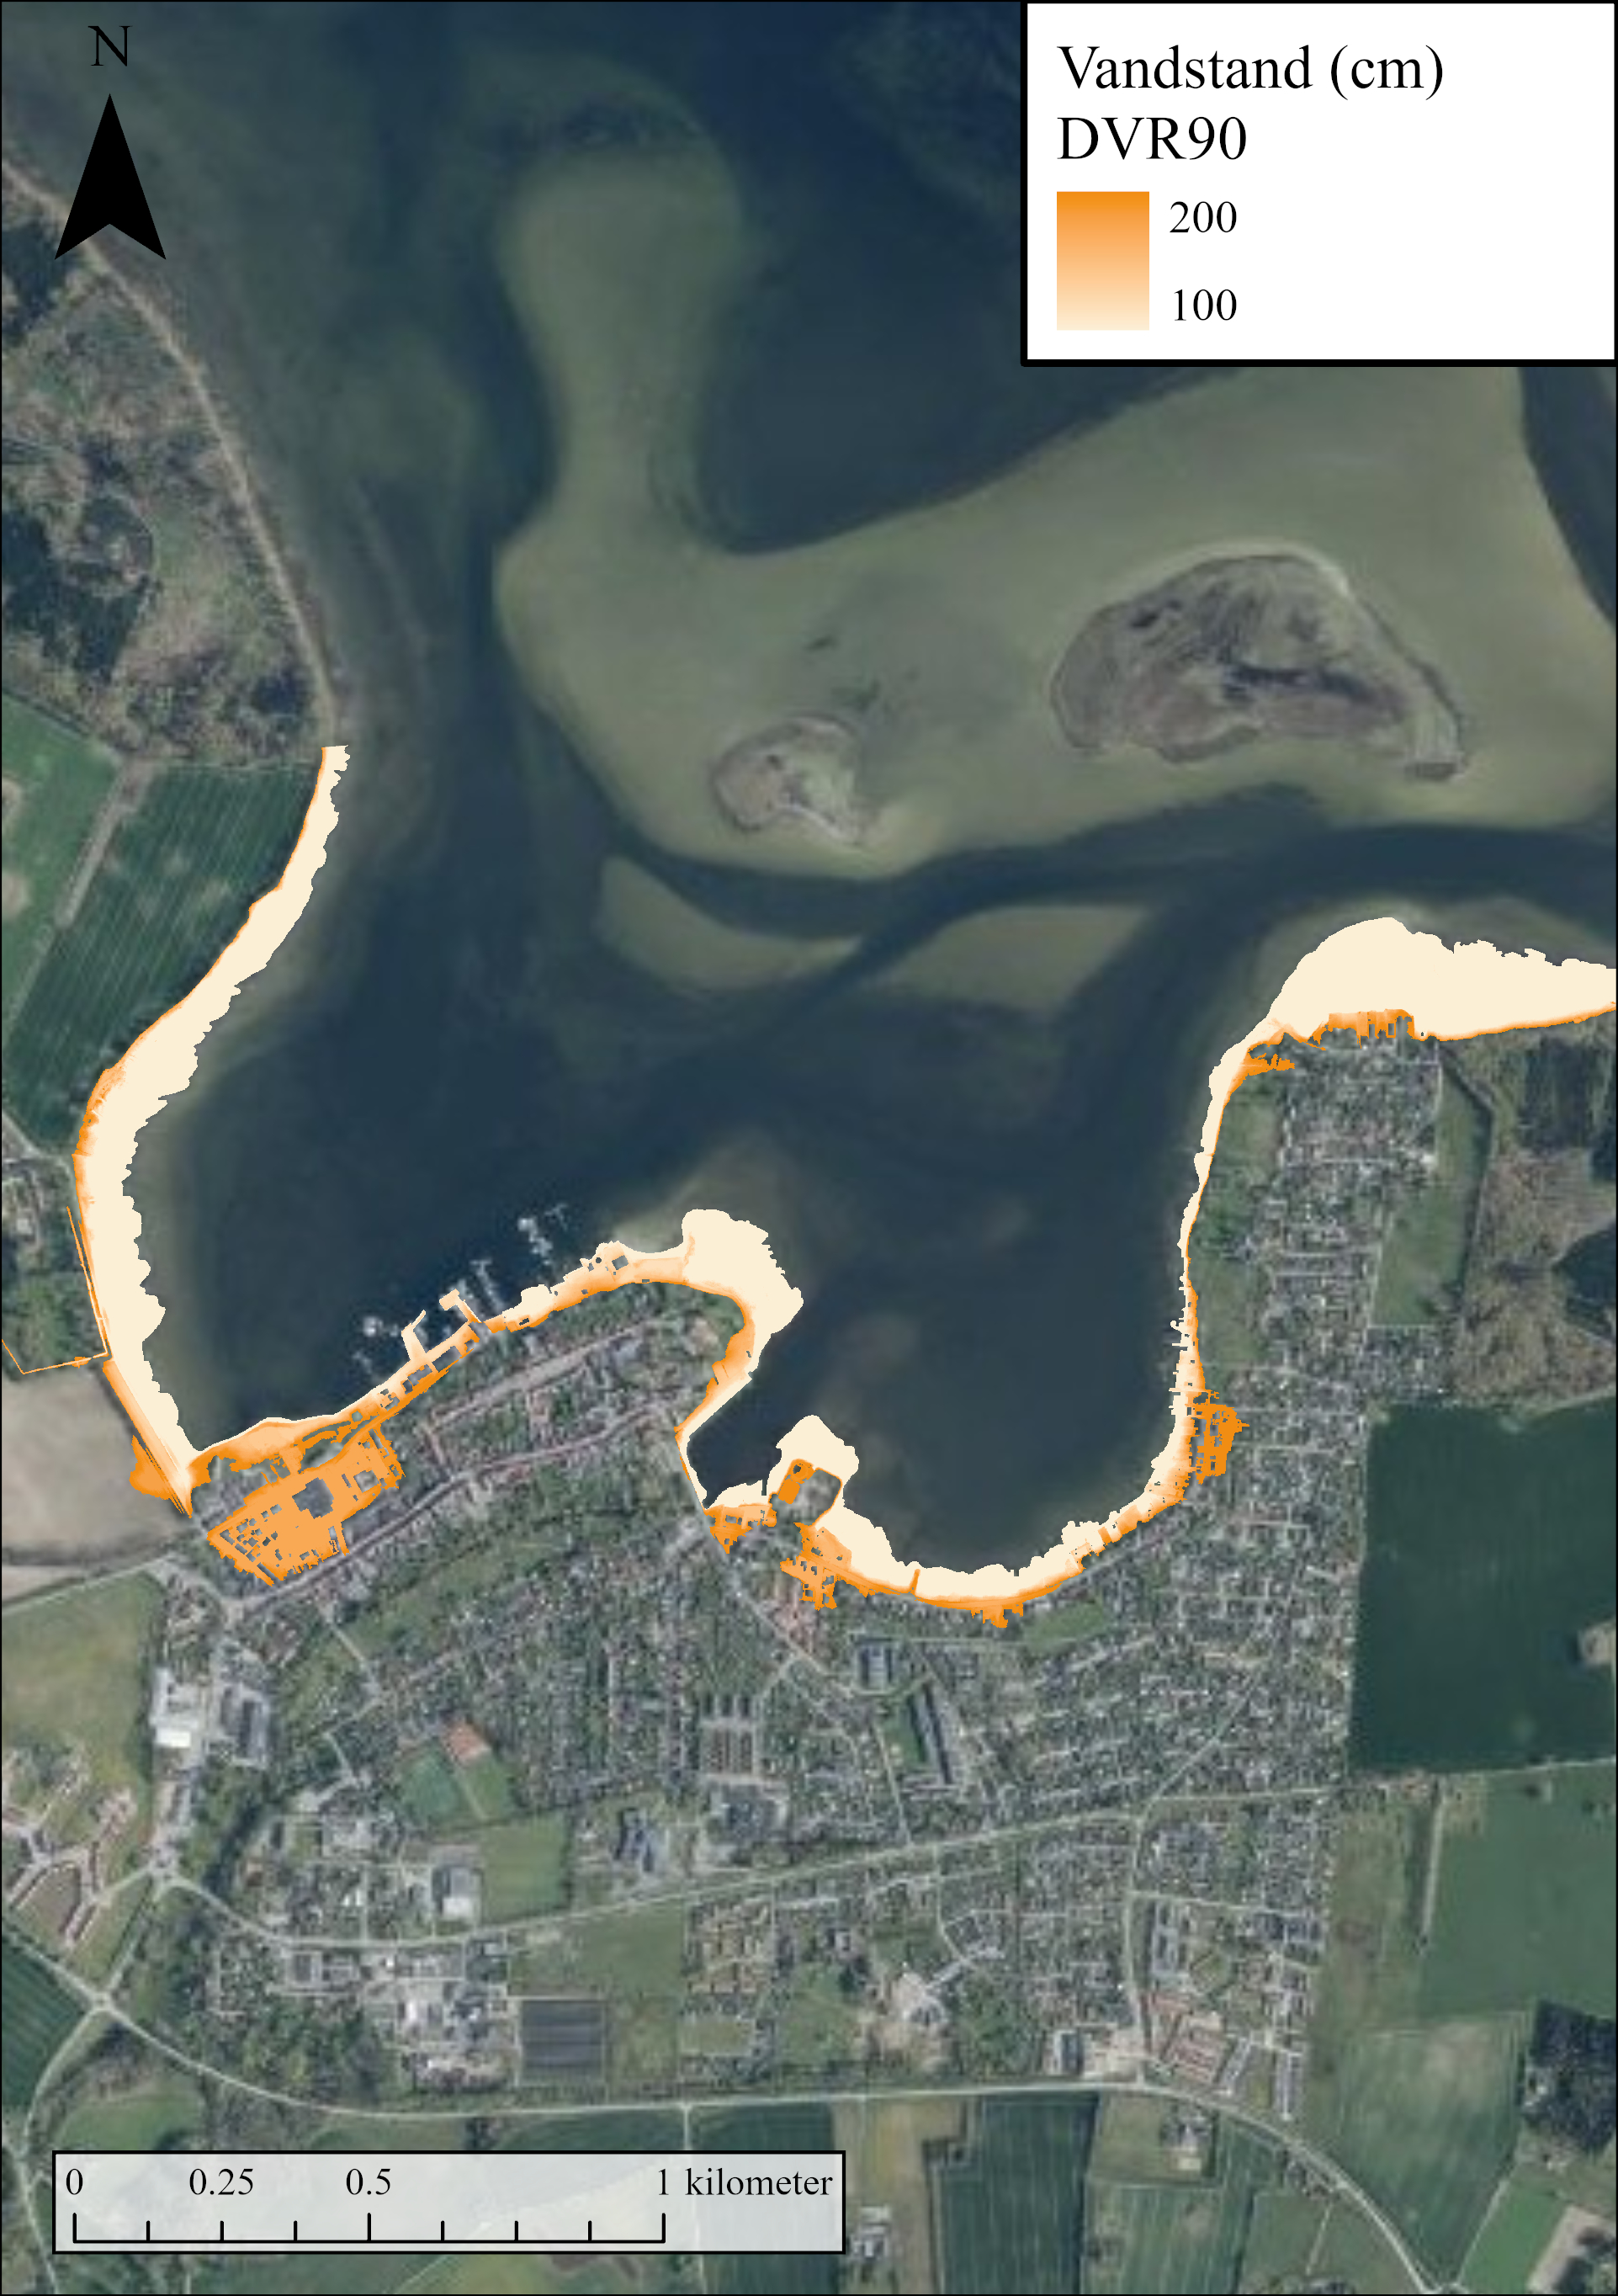
\includegraphics[width=0.95\linewidth]{images/Resultater/2023Model/2023 model_praestoe.jpg}
		\caption{}
		\label{Subfig: Model Præstø}
	\end{subfigure}
	\caption{Oversvømmelseskort over oktober 2023 stormfloden for Præstø. \textbf{(a)} Observeret data. \textbf{(b)} Simuleret data}
	\label{Figur: Målt & simuleret Præstø}
\end{figure}
Figure \ref{Figur: Målt & simuleret Præstø} shows the observed and simulated storm surge event for Præstø. Both maps show that the coast and harbour of Præstø become flooded at 2 metres, as well as the northern part of the town. The difference between the two maps are that during the actual storm surge, part of Tubæk Å and the surrounding areas were flooded. The observed event at 53.5 hectares is therefore 26\% larger in extent that the simulated result of 39.8 hectares. This difference amounts to 13.7 hectares.\\

\newpage
\subsection{Projected and 100-year storm surge events}
In this section a map of the projected storm surge based on the 2023 storm surge and a statistical 100 year event is presented.
\begin{figure}[H]
	\centering
	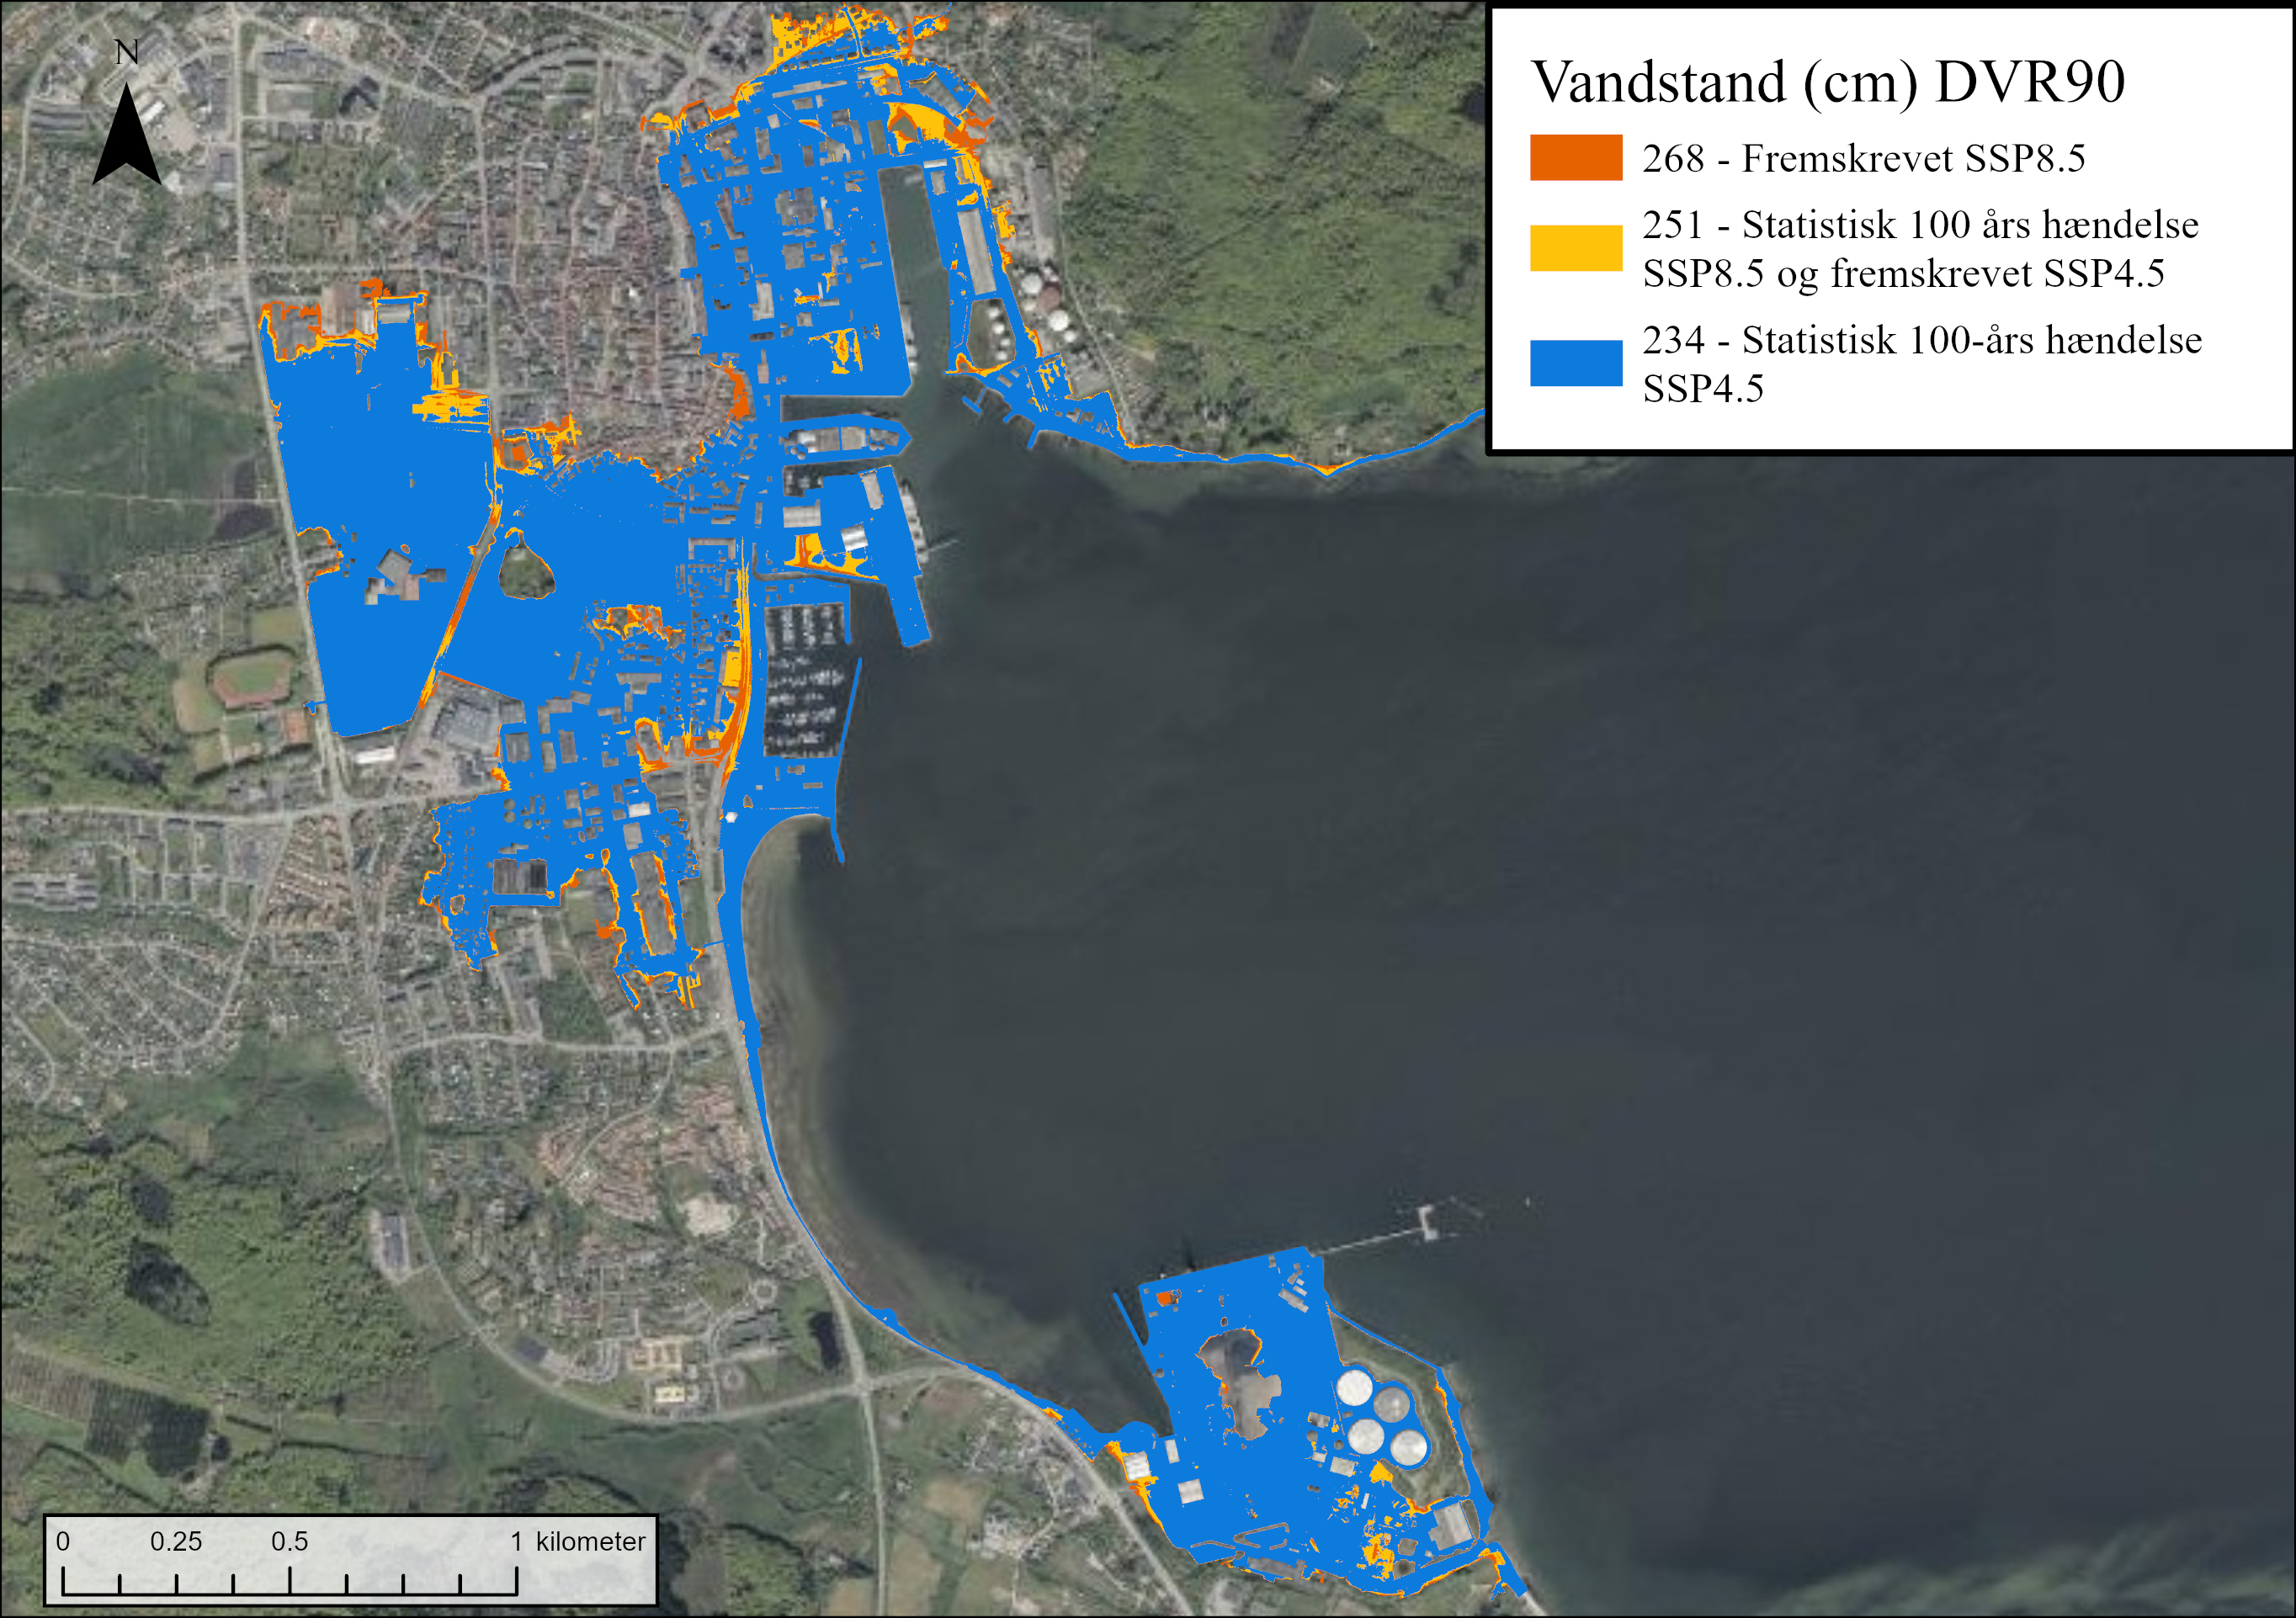
\includegraphics[width=0.8\linewidth]{images/Resultater/fremskrevet_hændelser/klima resultat_aabenraa.jpg}
	\caption{Kort over oversvømmet areal i Aabenraa af en stormflod ved en statistisk 100-års hændelse og en fremskrivning af 2023-stormfloden til slutningen af århundredet ved et SSP4,5 og SSP8,5 scenarie.}
	\label{Figur: Klima Aabenraa}
\end{figure}
Figure \ref{Figur: Klima Aabenraa} shows a flood map of Aabenraa for a 100-year event and a projetion of the 2023-storm surge for a SSP4.5 and SSP8.5 scenario. The largest flooding occurs for a 100-year event at SSP4.5 with a water level of 234 cm above DVR90, where a large part of the southern part of the main city centre is flooded. The flooded area for the projected 2023-storm surge in an SSP8.5 scenario is 13\% larger than the 100-year event at SSP4-5. A value that corresponds to 19.6 hectares. Compared to the observed storm surge in 2023, a projected storm surge floods an area of 96 and 104 hectares larger for SSP4.5 and SSP8.5, respectively. It is primarily the northern part of Aabenraa where there is a difference between the two projected events.
\begin{figure}[H]
	\centering
	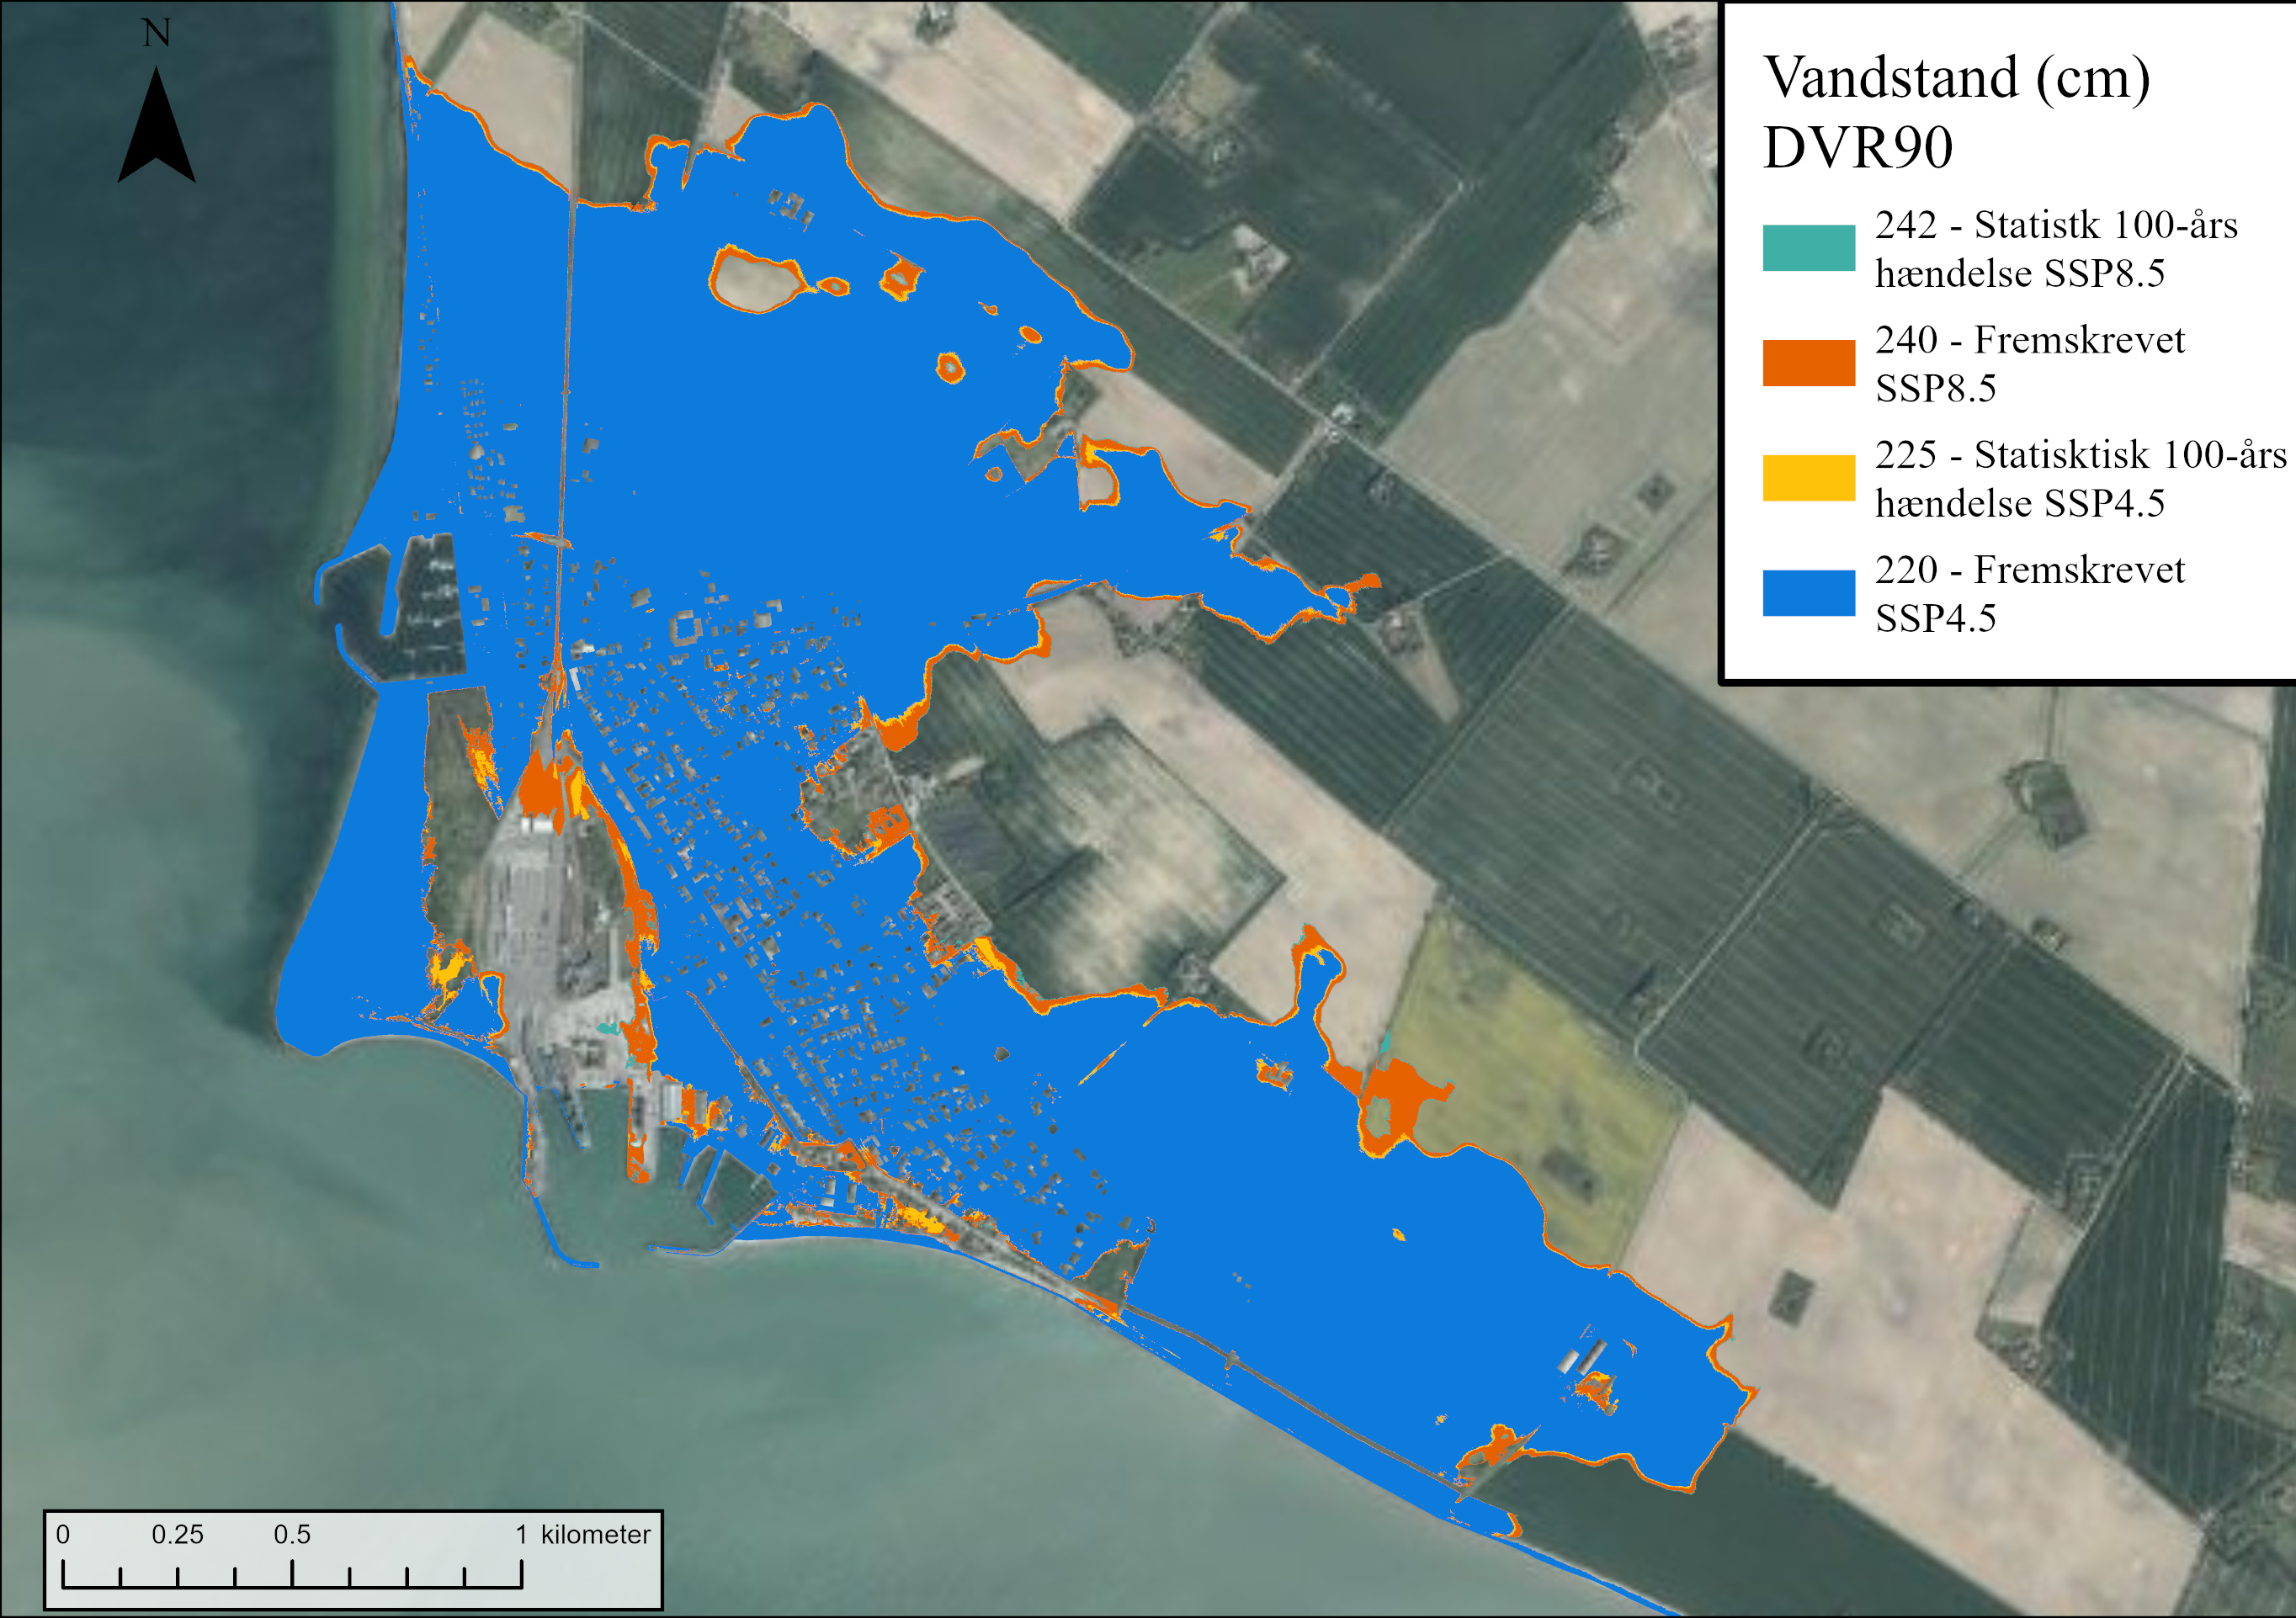
\includegraphics[width=0.8\linewidth]{images/Resultater/fremskrevet_hændelser/klima resultat gedser.jpg}
	\caption{Kort over oversvømmet areal i Gedser Havn af en stormflod ved en statistisk 100-års hændelse og en fremskrivning af oktober 2023 stormfloden til slutningen af århundredet ved et SSP4,5 og SSP8,5 scenarie.}
	\label{Figur: Klima Gedser Havn}
\end{figure}
Figure \ref{Figur: Klima Gedser Havn} shows the flood map of Gedser Havn for a 100-year event and a projection of the 2023-storm surge. The largest flooding occurs at a projected 2023-storm surge at SSP4.5 with a water level of 220 cm above DVR90. Most of the town is flooded as well as parts of the agricultural areas behind the town. For a 100-year event at SSP8.5, the total flooded area has increased to 219.7 hectares, an increase of 537\% compared to the storm surge that hit Gedser Havn in 2023. The inner parts of the ferry port and terminal will not be flooded in any of the four inundation scenarios, however, the main road to the ferry terminal will be flooded.
\begin{figure}[H]
	\centering
	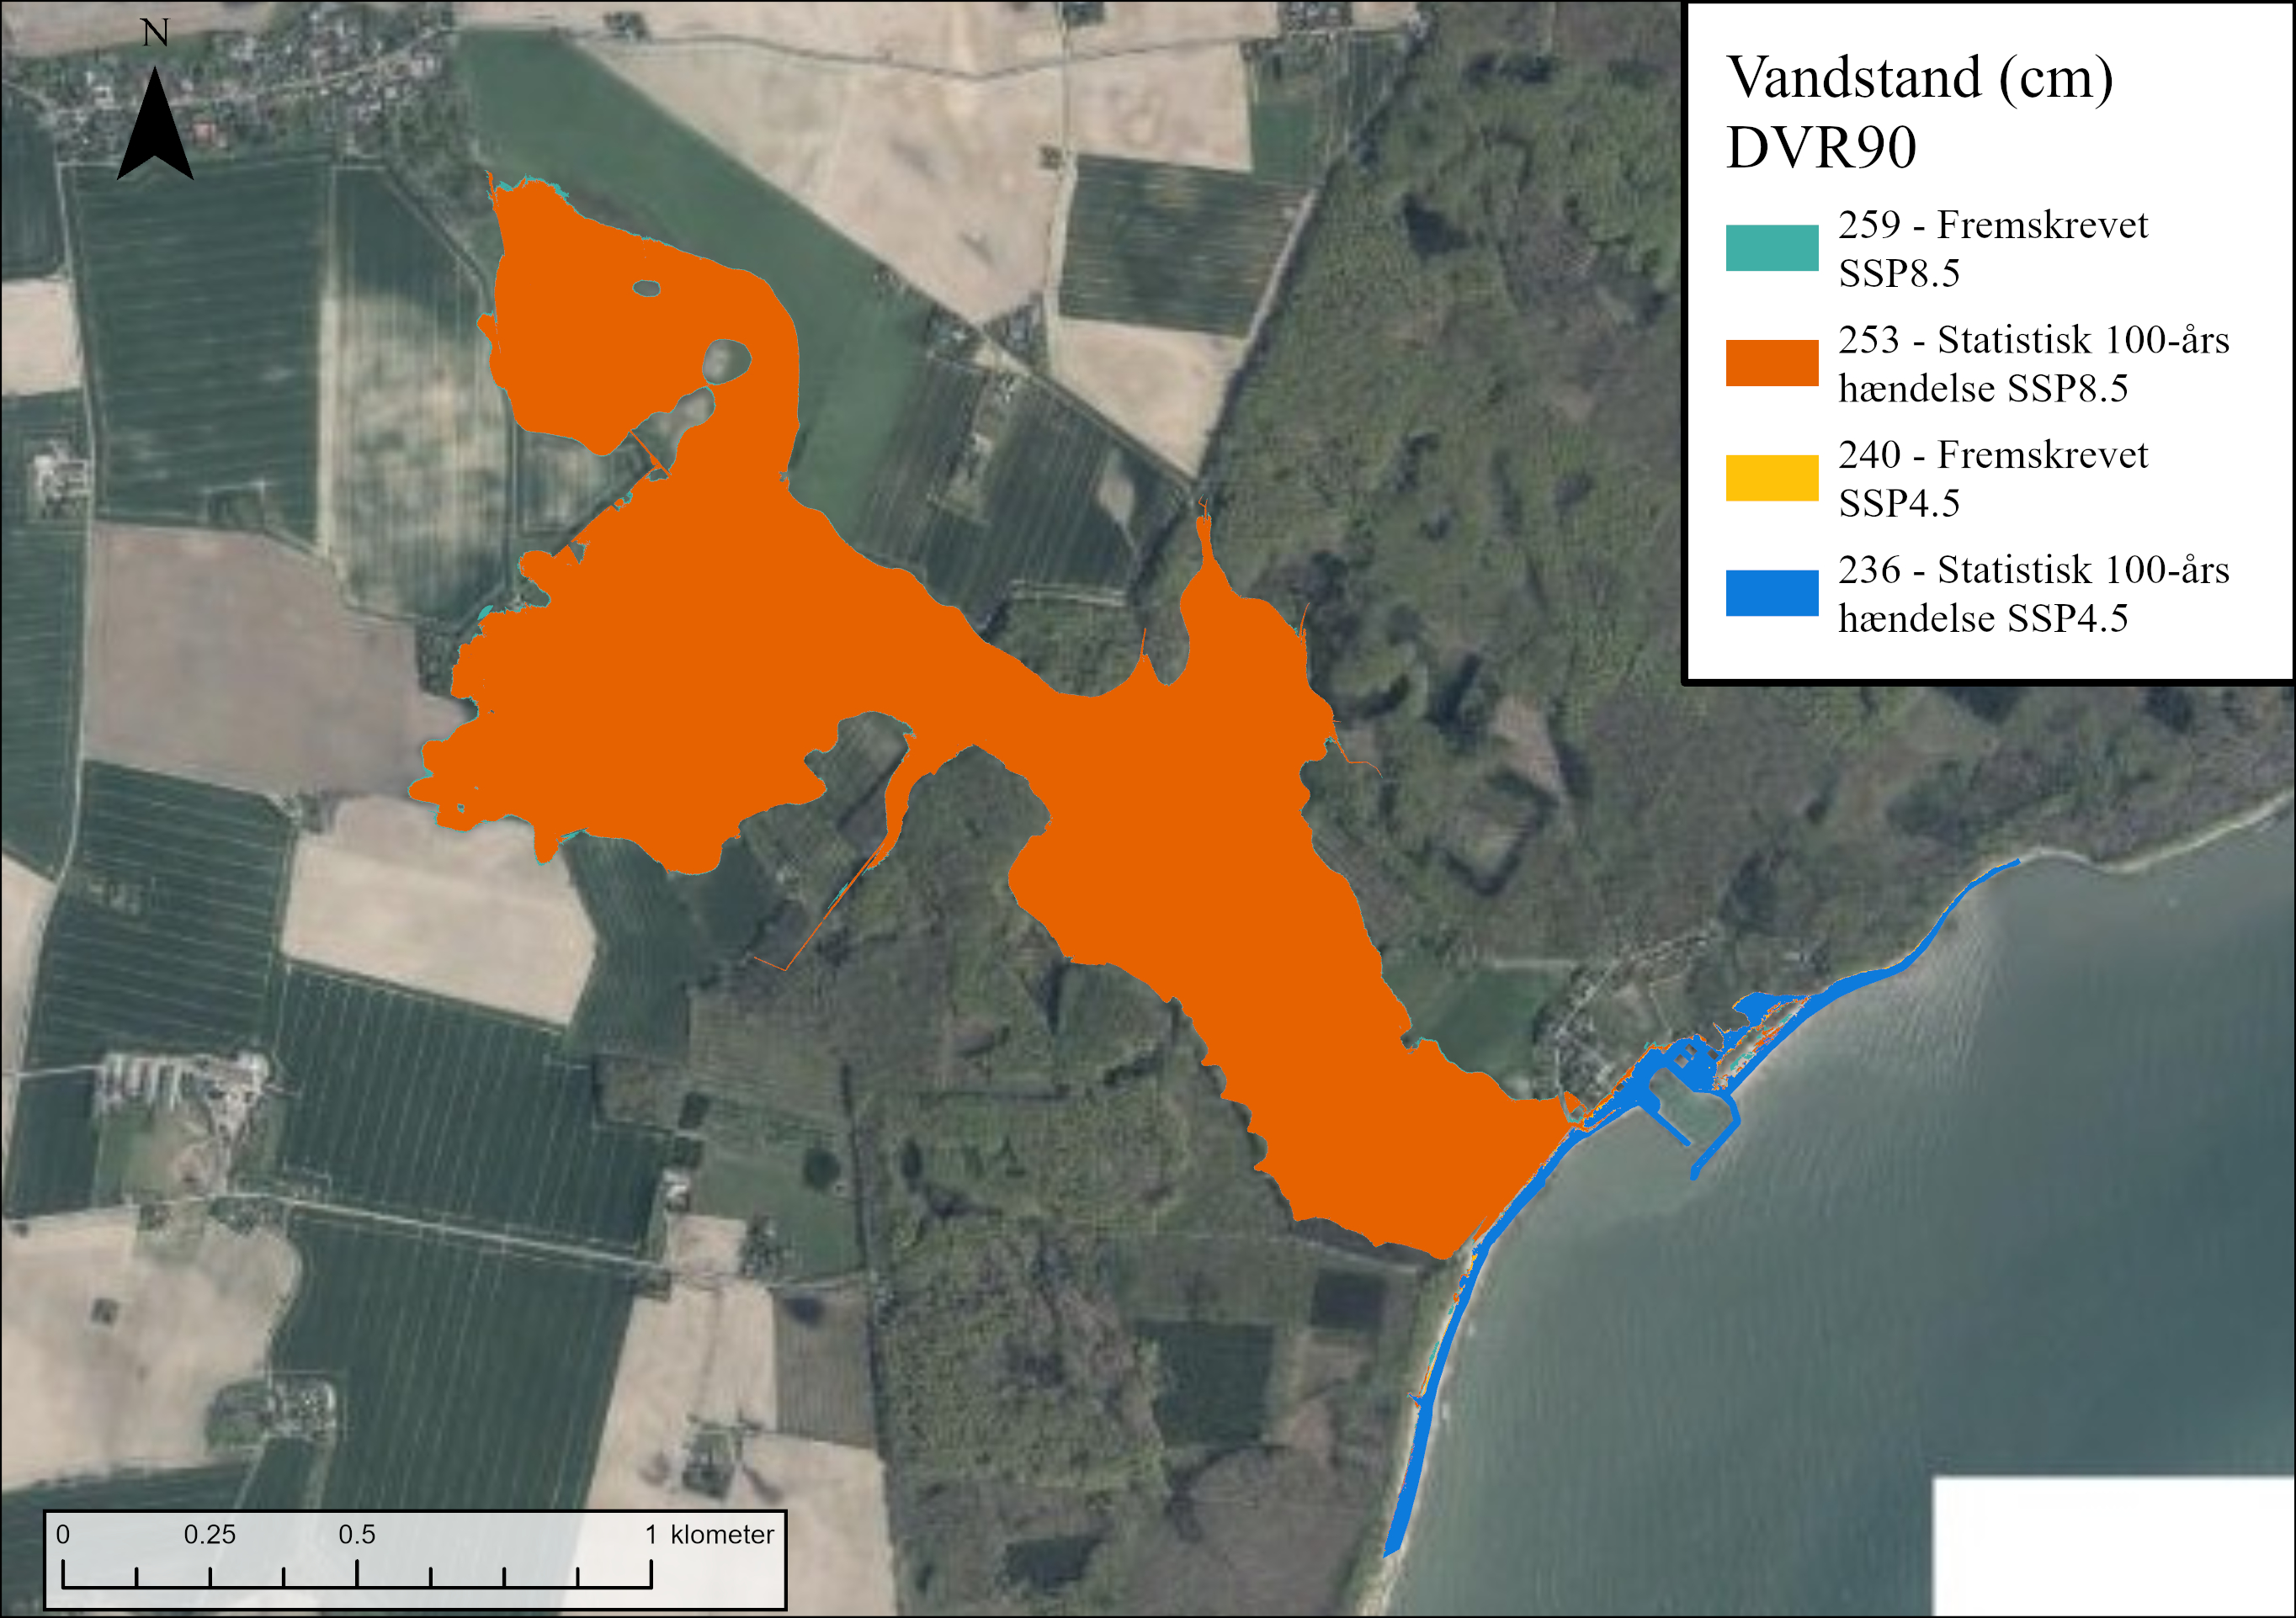
\includegraphics[width=0.8\linewidth]{images/Resultater/fremskrevet_hændelser/klima resultat hesnaes.jpg}
	\caption{Kort over oversvømmet areal i Hesnæs af en stormflod ved en statistisk 100-års hændelse og en fremskrivning af oktober 2023 stormfloden til slutningen af århundredet ved et SSP4,5 og SSP8,5 scenarie.}
	\label{Figur: Klima Hesnæs}
\end{figure}
In Hesnæs, a large low-lying area of mixed grassland and agriculture will be flooded in a 100-year event at SSP8.5. The town of Hesnæs itself is outside of the risk of flooding even at the highest water level of 259 cm DVR90 (Figure \ref{Figur: Klima Hesnæs}) due to the steep slope ascending from the harbour. In a projected 2023-storm surge at SSP8.5, the inundated area increased from 3.5 hectares to 114.8 hectares, amounting to an increase of 3219\%, or 111.3 hectares.\\

Figure \ref{Figur: Klima Præstø} shows the extent of the water during a 100-year storm surge event and a projection of the 2023-storm surge for Præstø. During the 100-event at SSP4.5, parts of Præstø town will be flooded. This accounts for areas both north and south of Tubæk Å. Most of the Tubæk Å valley will also be flooded and the stream itself will most likely overflow its banks in the south of the town. At water levels of more than 225 cm, the water will follow Tubæk Å further inland. An area that is 68\%, corresponding to 36 hectares, larger than the 2023-storm surge event will be flooded if the same storm surge hit Præstø at the end of this century at a SSP8.5 emission scenario.
\begin{figure}[H]
 	\centering
 	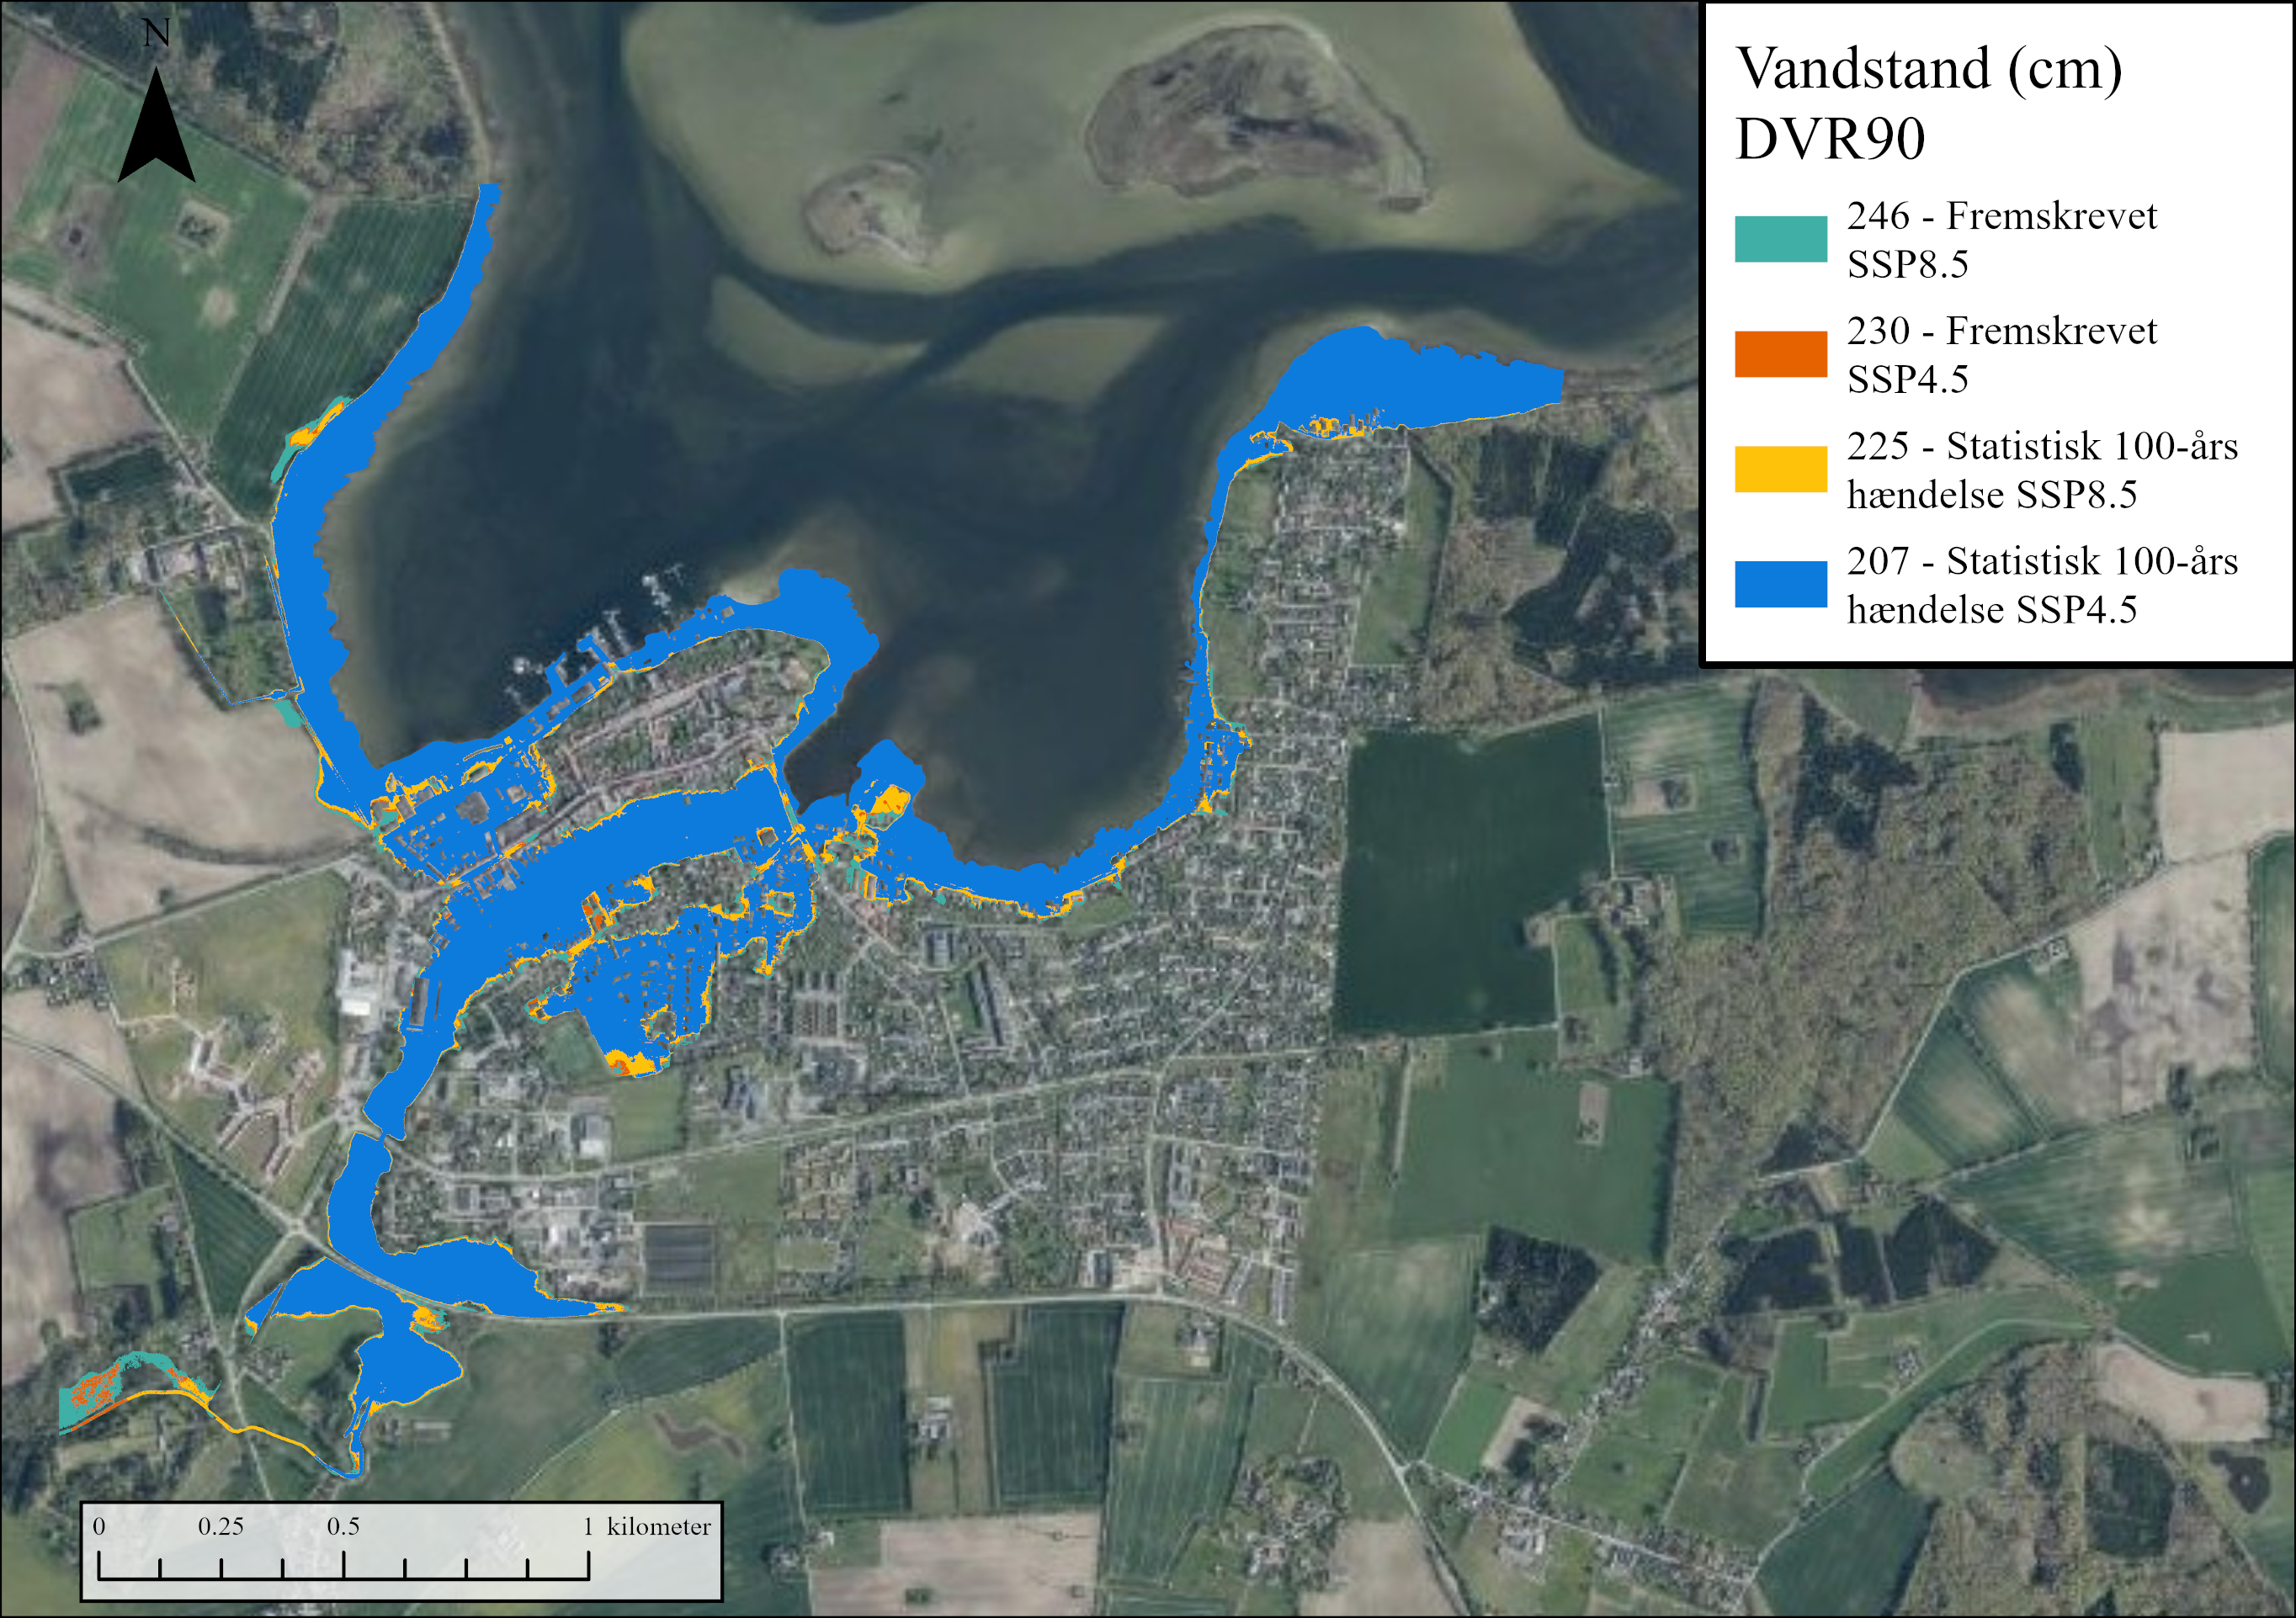
\includegraphics[width=0.8\linewidth]{images/Resultater/fremskrevet_hændelser/klima resultat praestoe.jpg}
 	\caption{Kort over oversvømmet areal i Præstø af en stormflod ved en statistisk 100-års hændelse og en fremskrivning af oktober 2023 stormfloden til slutningen af århundredet ved et SSP4,5 og SSP8,5 scenarie.}
 	\label{Figur: Klima Præstø}
\end{figure}
In summary, all four sites of interest are affected greatly by storm surge now and in the future. Table \ref{Tabel: Oversvømmet arealer af stormfloder} summarises the extent of the flooding in hectares for all simulated events and the observed storm surge from 2023. The largest flooded area is in Gedser Havn for a projected 2023-storm surge at SSP8.5 with an area of 219.7 hectares. While the smallest flooded area was the simulated result of the 2023-storm surge for Hesnæs with an inundated area of 3.3 hectares. Gedser Havn is also the area with the largest absolute increase in flooded area with an 183.6 hectare increase from the observed storm surge in 2023 to a projected flood of that storm surge in SSP8.5.
\begin{table}[H]
	\centering
	\renewcommand{\arraystretch}{1.2} 
	\begin{threeparttable}
		\caption{Oversvømmet areal af den observerede stormflod, den simuleret stormflod samt den statistiske 100-års hændelse og den fremskrevet stormflod til slutningen af århundredet ved SSP4.5 og 8.5 i hektar for hvert studieområde.}
		\begin{tabular}{@{} l S[table-format=3.1, output-decimal-marker={.}] 
				S[table-format=3.1, output-decimal-marker={.}] 
				S[table-format=3.1, output-decimal-marker={.}] 
				S[table-format=3.1, output-decimal-marker={.}] 
				S[table-format=3.1, output-decimal-marker={.}] 
				S[table-format=3.1, output-decimal-marker={.}] @{}} 
			\toprule
			& \multicolumn{1}{c}{\textbf{\makecell{Observed 2023\\storm surge}}} 
			& \multicolumn{1}{c}{\textbf{\makecell{Simulated 2023\\storm surge}}} 
			& \multicolumn{2}{c}{\textbf{\makecell{Statistical 100-year\\event}}} 
			& \multicolumn{2}{c}{\textbf{\makecell{Projected 2023\\storm surge}}} \\ 
			\cmidrule(l){4-5} \cmidrule(l){6-7}
			{\textit{hectares}} & & & {\textit{SSP4.5}} & {\textit{SSP8.5}} & {\textit{SSP4.5}} & {\textit{SSP8.5}} \\
			\midrule
			Aabenraa & 70.7 & 129.8 & 155.2 & 166.7 & 166.7 & 174.9 \\
			Gedser & 34.5 & 33.2 & 205.1 & 219.7 & 201 & 218.1 \\ 
			Hesnæs & 3.5 & 3.3 & 4.8 & 113.4 & 4.8 & 114.8 \\
			Præstø & 53.5 & 39.8 & 75.7 & 82 & 84.1 & 89.7 \\
			\bottomrule
		\end{tabular}
		\label{Tabel: Oversvømmet arealer af stormfloder}
	\end{threeparttable}
\end{table}